\documentclass{tfgitic}[2022/06/30]
\usepackage[version=4]{mhchem}
\usepackage{tikz}
\usepackage[europeanresistors,americaninductors]{circuitikz}
\usepackage{pgfplots}
\usepackage[plain,figure]{algorithm2e}
\usepackage{tabularx}
\usepackage{color}
\usepackage{listings}
\usepackage{comment}
\usepackage{array}
\usepackage{hhline}
\usepackage{colortbl}
\usepackage{tabularray}
\usepackage{longtable} 
\usepackage{fancyhdr}

\usetikzlibrary{arrows}
\addbibresource{docum-tfg.bib}
\setlength{\algomargin}{4em}
\pgfplotsset{compat=newest}
\newcommand*{\rom}[1]{\expandafter\@slowromancap\romannumeral #1@}

\definecolor{MineShaft}{rgb}{0.2,0.2,0.2}
\definecolor{Teal}{rgb}{0,0.501,0.501}
\definecolor{tufte1}{HTML}{B8B800}
\definecolor{yellowmarker}{HTML}{DEF440}
\definecolor{background}{RGB}{39, 40, 34}
\definecolor{string}{HTML}{4747ff}
\definecolor{comment}{RGB}{117, 113, 94}
\definecolor{normal}{RGB}{248, 248, 242}
\definecolor{identifier}{RGB}{166, 226, 46}
\definecolor{bgreen}{rgb}{0.0, 0.26, 0.15}
\definecolor{gray97}{rgb}{247, 247, 247}
\definecolor{blackred}{HTML}{581845}
\definecolor{blackpurple}{HTML}{c70039}
\definecolor{blackpink}{HTML}{900c3f}
\definecolor{royalblue}{HTML}{08298A}
\definecolor{veryroyalblue}{HTML}{5269AD}
\definecolor{cerceta}{HTML}{009B94}
\definecolor{PurpleNavy}{HTML}{4e5180}
\definecolor{LightCyan}{rgb}{0.88,1,1}

\lstdefinelanguage{CSS}{
  morekeywords={accelerator,azimuth,background,background-attachment,
    background-color,background-image,background-position,
    background-position-x,background-position-y,background-repeat,
    behavior,border,border-bottom,border-bottom-color,
    border-bottom-style,border-bottom-width,border-collapse,
    border-color,border-left,border-left-color,border-left-style,
    border-left-width,border-right,border-right-color,
    border-right-style,border-right-width,border-spacing,
    border-style,border-top,border-top-color,border-top-style,
    border-top-width,border-width,bottom,caption-side,clear,
    clip,color,content,counter-increment,counter-reset,cue,
    cue-after,cue-before,cursor,direction,display,elevation,
    empty-cells,filter,float,font,font-family,font-size,
    font-size-adjust,font-stretch,font-style,font-variant,
    font-weight,height,ime-mode,include-source,
    layer-background-color,layer-background-image,layout-flow,
    layout-grid,layout-grid-char,layout-grid-char-spacing,
    layout-grid-line,layout-grid-mode,layout-grid-type,left,
    letter-spacing,line-break,line-height,list-style,
    list-style-image,list-style-position,list-style-type,margin,
    margin-bottom,margin-left,margin-right,margin-top,
    marker-offset,marks,max-height,max-width,min-height,
    min-width,-moz-binding,-moz-border-radius,
    -moz-border-radius-topleft,-moz-border-radius-topright,
    -moz-border-radius-bottomright,-moz-border-radius-bottomleft,
    -moz-border-top-colors,-moz-border-right-colors,
    -moz-border-bottom-colors,-moz-border-left-colors,-moz-opacity,
    -moz-outline,-moz-outline-color,-moz-outline-style,
    -moz-outline-width,-moz-user-focus,-moz-user-input,
    -moz-user-modify,-moz-user-select,orphans,outline,
    outline-color,outline-style,outline-width,overflow,
    overflow-X,overflow-Y,padding,padding-bottom,padding-left,
    padding-right,padding-top,page,page-break-after,
    page-break-before,page-break-inside,pause,pause-after,
    pause-before,pitch,pitch-range,play-during,position,quotes,
    -replace,richness,right,ruby-align,ruby-overhang,
    ruby-position,-set-link-source,size,speak,speak-header,
    speak-numeral,speak-punctuation,speech-rate,stress,
    scrollbar-arrow-color,scrollbar-base-color,
    scrollbar-dark-shadow-color,scrollbar-face-color,
    scrollbar-highlight-color,scrollbar-shadow-color,
    scrollbar-3d-light-color,scrollbar-track-color,table-layout,
    text-align,text-align-last,text-decoration,text-indent,
    text-justify,text-overflow,text-shadow,text-transform,
    text-autospace,text-kashida-space,text-underline-position,top,
    unicode-bidi,-use-link-source,vertical-align,visibility,
    voice-family,volume,white-space,widows,width,word-break,
    word-spacing,word-wrap,writing-mode,z-index,zoom},
  morestring=[s]{:}{;},
  sensitive,
  morecomment=[s]{/*}{*/}
}
\lstdefinelanguage{JavaScript}{
  keywords={typeof, new, true, false, catch, function, return, null, catch, switch, var, if, in, while, do, else, case, break},
  keywordstyle=\color{blue}\bfseries,
  ndkeywords={class, export, boolean, throw, implements, import, this},
  ndkeywordstyle=\color{darkgray}\bfseries,
  identifierstyle=\color{black},
  sensitive=false,
  comment=[l]{//},
  morecomment=[s]{/*}{*/},
  commentstyle=\color{purple}\ttfamily,
  stringstyle=\color{red}\ttfamily,
  morestring=[b]',
  morestring=[b]"
}
\lstdefinelanguage{others}{
    keywords = {VirtualHost, ServerName, WSGIDaemonProces, user, group, threads, WSGIScriptAlias, Directory, ErrorLog, certbot, systemctl},
    keywordstyle = \color{bgreen}\bfseries,
    ndkeywords = {ls, cat, cd, rm, mv, A2enmod, sudo, service, local, ssh},
    ndkeywordstyle = \color{magenta}\bfseries,
    identifierstyle = \color{black},
    sensitive = false,
    comment = [l]{#},
    commentstyle = \color{comment}\ttfamily,
    morestring=[b]',
    morestring=[b]"
}
\lstdefinestyle{bash}{
    language=others,
    numbers=none,
    backgroundcolor=\color[HTML]{ffffff}, %\color{background},
    showspaces=false,
    showstringspaces=false,
    aboveskip = 10px,
    showtabs=false,
    tabsize=4,
    captionpos=b,
    breaklines=true,
    breakatwhitespace=true,
    title=\lstname,
    basicstyle=\color{black}\footnotesize\sffamily,
    keywordstyle=\color{magenta}\footnotesize\sffamily\bfseries, % bgreen 
    stringstyle=\color{royalblue}\footnotesize\sffamily,
    commentstyle=\color{comment}\footnotesize,\sffamily,
    emph={format_string, eff_ana_bf, permute, eff_ana_btr},
    emphstyle=\color{PurpleNavy}\footnotesize\sffamily,
}
\lstdefinestyle{html}{
    language=html,
    numbers=none,
    backgroundcolor=\color[HTML]{ffffff}, %\color{background},
    showspaces=false,
    showstringspaces=false,
    aboveskip = 10px,
    showtabs=false,
    tabsize=4,
    captionpos=b,
    breaklines=true,
    breakatwhitespace=true,
    title=\lstname,
    basicstyle=\color{black}\footnotesize\sffamily,
    stringstyle=\color{royalblue}\footnotesize\sffamily,
    commentstyle=\color{comment}\footnotesize,\sffamily,
    emph={format_string, eff_ana_bf, permute, eff_ana_btr},
    emphstyle=\color{PurpleNavy}\footnotesize\sffamily,
    keywordstyle=\color{magenta}\footnotesize\sffamily\bfseries, % bgreen 
}
\lstdefinestyle{python}{
    language=python,
    numbers=none,
    backgroundcolor=\color[HTML]{ffffff}, %\color{background},
    showspaces=false,
    showstringspaces=false,
    aboveskip = 10px,
    showtabs=false,
    tabsize=4,
    captionpos=b,
    breaklines=true,
    breakatwhitespace=true,
    title=\lstname,
    basicstyle=\color{black}\footnotesize\sffamily,
    stringstyle=\color{royalblue}\footnotesize\sffamily,
    commentstyle=\color{comment}\footnotesize,\sffamily,
    emph={format_string, eff_ana_bf, permute, eff_ana_btr},
    emphstyle=\color{PurpleNavy}\footnotesize\sffamily,
    keywordstyle=\color{magenta}\footnotesize\sffamily\bfseries, % bgreen 
}
\lstdefinestyle{javascript}{
    language=JavaScript,
    numbers=none,
    backgroundcolor=\color[HTML]{ffffff}, %\color{background},
    showspaces=false,
    showstringspaces=false,
    aboveskip = 10px,
    showtabs=false,
    tabsize=4,
    captionpos=b,
    breaklines=true,
    breakatwhitespace=true,
    title=\lstname,
    basicstyle=\color{black}\footnotesize\sffamily,
    stringstyle=\color{royalblue}\footnotesize\sffamily,
    commentstyle=\color{comment}\footnotesize,\sffamily,
    emph={format_string, eff_ana_bf, permute, eff_ana_btr},
    emphstyle=\color{PurpleNavy}\footnotesize\sffamily,
    keywordstyle=\color{magenta}\footnotesize\sffamily\bfseries, % bgreen 
}
\lstdefinestyle{sql}{
    language=sql,
    numbers=none,
    backgroundcolor=\color[HTML]{ffffff}, %\color{background},
    showspaces=false,
    showstringspaces=false,
    aboveskip = 10px,
    showtabs=false,
    tabsize=4,
    captionpos=b,
    breaklines=true,
    breakatwhitespace=true,
    title=\lstname,
    basicstyle=\color{black}\footnotesize\sffamily,
    keywordstyle=\color{royalblue}\footnotesize\sffamily\bfseries, % bgreen 
    stringstyle=\color{bgreen}\footnotesize\sffamily,
    commentstyle=\color{comment}\footnotesize,\sffamily,
    emph={format_string, eff_ana_bf, permute, eff_ana_btr},
    emphstyle=\color{PurpleNavy}\footnotesize\sffamily,
}
\lstdefinestyle{css} {%
  language=CSS,
  basicstyle={\footnotesize\sffamily},   
  showspaces = false,
  showstringspaces = false,
  showtabs = false,
  numbers=none,
  identifierstyle=\color{royalblue},
  keywordstyle=\color{magenta}\sffamily,
  ndkeywordstyle=\color{royalblue}\sffamily,
  stringstyle=\color{cerceta}\sffamily,
  commentstyle=\color{comment}\sff,
  alsodigit={.:;},	
  showtabs=false,
  extendedchars=true,
  breaklines=true,
}
\lstset{literate=
  {á}{{\'a}}1 {é}{{\'e}}1 {í}{{\'i}}1 {ó}{{\'o}}1 {ú}{{\'u}}1
  {Á}{{\'A}}1 {É}{{\'E}}1 {Í}{{\'I}}1 {Ó}{{\'O}}1 {Ú}{{\'U}}1
  {à}{{\`a}}1 {è}{{\`e}}1 {ì}{{\`i}}1 {ò}{{\`o}}1 {ù}{{\`u}}1
  {À}{{\`A}}1 {È}{{\'E}}1 {Ì}{{\`I}}1 {Ò}{{\`O}}1 {Ù}{{\`U}}1
  {ä}{{\"a}}1 {ë}{{\"e}}1 {ï}{{\"i}}1 {ö}{{\"o}}1 {ü}{{\"u}}1
  {Ä}{{\"A}}1 {Ë}{{\"E}}1 {Ï}{{\"I}}1 {Ö}{{\"O}}1 {Ü}{{\"U}}1
  {â}{{\^a}}1 {ê}{{\^e}}1 {î}{{\^i}}1 {ô}{{\^o}}1 {û}{{\^u}}1
  {Â}{{\^A}}1 {Ê}{{\^E}}1 {Î}{{\^I}}1 {Ô}{{\^O}}1 {Û}{{\^U}}1
  {ã}{{\~a}}1 {ẽ}{{\~e}}1 {ĩ}{{\~i}}1 {õ}{{\~o}}1 {ũ}{{\~u}}1
  {Ã}{{\~A}}1 {Ẽ}{{\~E}}1 {Ĩ}{{\~I}}1 {Õ}{{\~O}}1 {Ũ}{{\~U}}1
  {œ}{{\oe}}1 {Œ}{{\OE}}1 {æ}{{\ae}}1 {Æ}{{\AE}}1 {ß}{{\ss}}1
  {ű}{{\H{u}}}1 {Ű}{{\H{U}}}1 {ő}{{\H{o}}}1 {Ő}{{\H{O}}}1
  {ç}{{\c c}}1 {Ç}{{\c C}}1 {ø}{{\o}}1 {å}{{\r a}}1 {Å}{{\r A}}1
  {€}{{\euro}}1 {£}{{\pounds}}1 {«}{{\guillemotleft}}1
  {»}{{\guillemotright}}1 {ñ}{{\~n}}1 {Ñ}{{\~N}}1 {¿}{{?`}}1 {¡}{{!`}}1 
}

\title{Millora d'un sistema de recol·lecció de dades}
\subtitle{Migració de la plataforma a Raspberry Pi i millora de l'API}
\author{Francesc Arrufí Fernández}
\advisor{Jordi Bonet Dalmau}

\dedication{
\emph{<<One day a tortoise will learn how to fly.>>}\\
\acro{Terry Pratchett}\\
--- Small Gods
}

\begin{acknowledgments}
Als meus pares, que m'han fet costat sempre de forma incondicional.

A Ingimec, que m'ha permès fer el meu treball de fi de grau dins la seva empresa i en tot moment s'ha mostrat comprensiva i atenta.

Als meus professors, i en especial al director d'aquest treball, Jordi Bonet Dalmau, per aguantar totes les preguntes que li he fet, inclús les més banals.

Als meus companys de carrera, en David Comabella, en Joan Marc Serrano i en Jordi Salguero, amb vosaltres he fet quasi totes les assignatures i pràctiques i si estic ara aquí és pel vostre suport. També a tots aquells estudiants que m'han ajudat en moments puntuals, com en Hafid o en Toni Sbert. Sense tots ells ara no seria aquí, i per això us dono els més sincers agraïments.

I en especial al meu tiet, el Dr. Manuel Fernández López, que m'ha donat tota la seva experiència d'una vida dedicada a la investigació i la docència. T'estic molt agraït.
\end{acknowledgments}

\begin{resum}
Any 2019: Ingimec rep l'encàrrec d'un client de Polònia. S'ha de crear un sistema de visualització de dades per a una de les seves línies. Ingimec encarrega el projecte a una altra empresa. Neix el projecte $4246$.

Any 2020: a l'empresa no agrada el resultat d'aquesta decisió. Decideix deixar el projecte al seu departament encarregat de la programació dels equips que controlen les línies de producció que dissenya. Aquest decideix continuar aplicant les mateixes tecnologies que l'empresa externa. Arriba l'any vint-i-u i el projecte s'acaba abandonant a causa de canvis en l'estructura del departament i l'ocasional falta de personal.

Any 2022: arriben noves incorporacions al departament. Es decideix enfocar el projecte des d'un altre prisma. Ara ja no és un encàrrec per a un client, és un esquer que ha de permetre captar-ne de nous. S'apliquen millores i canvis i s'implementa un prototip en un entorn industrial.

Any 2023: els costos derivats de les decisions tècniques anteriors fan inviable el projecte. Es decideix començar de zero i trencar amb tot el treball previ. Abans era Azure, ara és Flask. Anteriorment era una \acro{esp$32$} amb entrades i sortides físiques i limitades, ara és una Raspberry Pi amb wifi que es comunica amb els \acro{plc} mitjançant Ethernet. Era C#, \acro{.net} i Model-Vista-Controlador; ara és Python, \acro{html} i JavaScript. A l'inici es basava en els productes de Microsoft, ara es basa en Linux i codi obert.

Hi ha molts projectes amb un objectiu semblant. Formes increïbles de fer-los. Maneres totalment oposades de crear una mateixa cosa. Aquest és un projecte de tants, fet d'una altra manera.

Aquest és el meu treball de fi de grau.
\end{resum}

\begin{abstract}
Year 2019: Ingimec receives an order from a customer in Poland. A data display system must be created for one of their production lines. Ingimec entrusts the project to an external company, and the $4246$ project is born.

Year 2020: Ingimec is not satisfied with the outcome of the external company's work, so they decide to assign the project to their in-house programming department responsible for designing and programming the production lines. This department decides to continue using the same technologies as the external company. However, due to changes in the department's structure and occasional lack of staff, the project is eventually abandoned.

Year 2022: With new additions to the company, they decide to approach the project from a different perspective. Instead of being solely an order for a customer, the project is seen as an opportunity to attract new customers. Improvements and changes are made, and a prototype is implemented in an industrial environment.

Year 2023: The costs associated with previous technical decisions make the project unfeasible. It is decided to start from scratch and break with all previous work. Previously based on Azure, now it is based on Flask. Previously using an \acro{esp$32$} with limited physical inputs and outputs, now they use a Desbarra with Wi-Fi that communicates with \acro{plc}s via Ethernet. It was previously developed with C#, \acro{.NET}, and Model-View-Controller, and now it uses Python, \acro{html}, and JavaScript. Initially based on Microsoft products, now it is based on Linux and open-source technologies.

There are many projects with a similar goal. Amazing ways to make them. Totally opposite ways of creating the same thing. This is a project of many, done in a different way.

This is my graduation thesis.
\end{abstract}

\begin{document}
\listoffigures\listoftables

% Si feu servir apendix, desomenteu.
\part{Memòria}

%%%%%%%%%%%%%%%%%%%%%%%%%%%%%%%%%%%%%%%%%%%%%%%%%
\chapter{Introducció}
Ingimec va ser contractada el 2019 per dotar un dels seus productes d'un sistema eficaç de
visualització de dades, estil els quadres de comandament que s'acostumen a veure en les plantes
de producció. Segons el client, aquest sistema havia d'estar basat en el núvol, mostrar les dades
de les diverses màquines de la línia de producció en una interfície web amigable i adaptativa,
calcular l'efectivitat total dels equips i guardar-ho tot en una base de dades. Naixia així el
projecte 4246.

En aquell moment es va decidir subcontractar una empresa externa per al seu disseny i
implementació, la qual va decidir basar-ho tot en la plataforma Microsoft Azure. Azure és una
plataforma basada en el núvol creada per Microsoft i que ofereix, entre d'altres, sistemes de
computació al núvol, gestió de dades, accés a servidors, emmagatzematge... La gestió de dades
estaria basada en Cosmos \acro{DB}, un servei també creat per Microsoft que ofereix bases de dades
distribuïdes. Això no obstant, totes aquestes decisions van comportar, a la llarga, un sobrecost
inesperat perquè entre molts altres factors Azure basa la seva tarifa en el nombre de
transaccions que es fan, de forma que el cost s'anava incrementant com més dades s'enviaven
al servidor.

Posteriorment, Ingimec es va adonar que aquesta no era la millor solució: dependre
d'una empresa externa com Microsoft, amb un sistema que plantejava uns costos poc raonables
per un projecte com aquest, obligava a encarir el preu final del producte que es volia vendre.
Des d'un principi aquest projecte es va plantejar com un afegit a les màquines fabricades i
dissenyades per l'empresa que tindria de captar futurs clients. Per fer-ho, el sistema ideat
hauria de ser flexible, ampliable i barat, i aquests objectius no es complirien en un sistema
com l'inicialment plantejat.

És per aquest motiu que ara s'ha decidit començar el projecte de nou, basant-ho tot en
plataformes i sistemes lliures i preferiblement de codi obert. Per fer-ho, s'han plantejat diversos
canvis que obliguen a dissenyar-ho tot des de zero. Ara, la base de dades Cosmos DB s'ha
canviat per una base de dades SQLite3 que res té a veure amb l'anterior; les comunicacions
entre els \acro{plc} que controlen les màquines i el servidor, inicialment plantejades per funcionar
amb una esp32, ara s'han canviat per unes més simples programades amb Python; un servidor
Flask i una aplicació web creats des de zero substitueixen el servidor d'Azure i els càlculs que
es volien calcular i visualitzar s'han replantejat i modificat per fer-los més robustos de cara al
futur. Una Raspberry PI ha de fer de nexe entre tots aquests punts.

Aquest treball recull tot aquest procés, el de migració d'una plataforma privativa i amb
uns costos desproporcionats per un sistema creat des de zero per Ingimec, flexible i basat en
codi obert. Des de la planificació de les tecnologies emprades i els càlculs realitzats, fins a la
implementació final — que compren tant l'emmagatzematge de les dades, les comunicacions
amb els \acro{plc} que controlen la maquinària dissenyada internament i l'execució dels càlculs plantejats com el disseny i implementació del servidor Flask i la interfície Web — es recullen en un
document que mostra tot el treball fet i que poc té a veure amb uns objectius similars
però implementats des d'un altre prisma totalment diferent.

%%%%%%%%%%%%%%%%%%%%%%%%%%%%%%%%%%%%%%%%%%%%%%%%%
\chapter{Antecedents}
L'origen d'aquest treball és el projecte 4246 d'Ingimec, el qual ha anat passant de mans i que mai s'ha acabat de definir. L'objectiu inicial d'aquest projecte és la creació d'un sistema de control visual accessible des de qualsevol entorn web, així com la consegüent creació d'una base de dades i d'un sistema de control/configuració en temps real.

\begin{figure}[h]
\centering
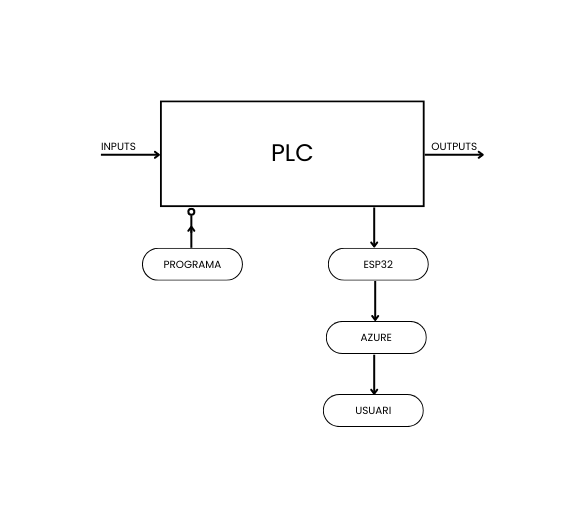
\includegraphics[width=0.5\textwidth]{img/diagramAzure.png}
\caption{En la primera implementació, es va fer servir una ESP32 per enviar les dades a un servidor basat en els serveis de Microsoft. L'\acro{esp32} recollia les dades mitjançant les seves limitades entrades i sortides digitals i les enviava al servidor de Microsoft mitjançant wifi.} 
\label{diagramAzure}
\end{figure}

La primera implementació — Figura \ref{diagramAzure} — d'aquest projecte és la creació d'un sistema
Azure coexistent a una base de dades Cosmos DB. Cosmos DB és una base de dades noSQL
distribuïda lligada intrínsecament a la plataforma de computació des del núvol Azure, ambdós
implementats per Microsoft. Això permet una ràpida configuració inicial, tot i que lligada als
productes de Microsoft. El fet que aquestes plataformes no són lliures i que el seu cost ve
determinat arbitràriament pels desitjos de Microsoft, han fet inviable continuar en aquesta
direcció.

En Azure, el servei d'emmagatzematge de BLOB té un cost associat amb la transferència
de dades, que es basa en la quantitat de dades transferides, així com en la ubicació geogràfica
d'aquestes. A més, també hi ha costos associats amb la transferència de dades a través de les
xarxes virtuals d'Azure, com en el tràfic sortint des d'una xarxa virtual a Internet \cite{azure:bandwidth-pricing}.

Amb aquest sistema, les dades s'envien a través d'un dispositiu basat en un ESP32 i desenvolupat per l'empresa bagenca Industrial Shields que envia les dades que recull a través de
les seves entrades digitals cap al servidor Azure mitjançant una connexió wifi.
A causa de la limitació física que té aquest dispositiu en comptar amb entrades digitals limitades,
i als costos comentats anteriorment, s'ha optat per implementar una segona opció.

\begin{figure}[h]
\centering
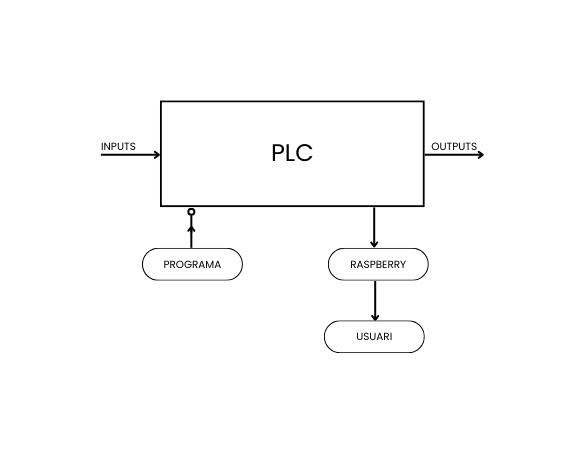
\includegraphics[width=0.5\textwidth]{img/diagramRaspberry.png}
\caption{La segona implementació, en canvi, treu els serveis de Microsoft i l'ESP32 i ho canvia directament per una Raspberry PI que fa totes dues funcions. Aquest dispositiu llegeix les dades del \acro{plc} mitjançant Ethernet, i disposa d'un segon port a més de wifi per si es vol activar la connexió a Internet amb un sistema o altre}
\label{diagramRaspberry}
\end{figure}

La segona implementació --- Figura \ref{diagramRaspberry} ---, recollida en aquest treball, ha estat la creació del mateix sistema a través d'un servidor Linux allotjat en una Raspberry PI. S'ha optat per una Raspberry PI degut al seu poc cost i a que és un sistema que conté potència suficient per a complir l'objectiu proposat. En aquest punt, la connexió amb els \acro{plc} és a través d'Ethernet, el qual és més potent que les entrades digitals del dispositiu d'Industrial Shields. Això també permet una connexió directa amb els \acro{plc}, així com una major flexibilitat i escalabilitat de cara al futur. D'aquesta forma, si es vol millorar i afegir funcionalitats al sistema només s'ha d'incrementar el bus de bytes enviats des del \acro{plc} o canviar la Raspberry PI per un ordinador més potent.

Com es pot observar, el primer camí i el segon no són compatibles. Això comporta que s'hagi de tornar a fer tot de nou, començant des de la tramesa de dades del \acro{plc} cap a la Raspberry, passant per la creació de la base de dades i acabant amb el servidor Web allotjat en la mateixa Raspberry PI.

%%%%%%%%%%%%%%%%%%%%%%%%%%%%%%%%%%%%%%%%%%%%%%%%%/
\chapter{Càlculs, requeriments i competència}
\label{Chapter: CalcReqCom}
\section{Càlculs}
\label{section:oee}
La finalitat d'aquest projecte és proporcionar un sistema de visualització atractiu i en temps real del rendiment d'una fàbrica, i per fer-ho és necessari calcular l'\acro{oee}. Aquest és un index percentual que mesura la productivitat de les fàbriques mitjançant tres paràmetres: disponibilitat, rendiment i qualitat. Descrit per primer cop per Seiichi Nakajima el 1982 en un article en japonès anomenat \emph{TPM tenkai} i publicat per l'Institut Japonès de Manteniment de Plantes (JIPM)\cite{IntangibleCapital:tpm01} i posteriorment editat en anglès \cite{Nakajima:tpm01}, és l'indicador més acceptat per mesurar l'eficiència i productivitat d'una planta.

\subsection{Disponibilitat}
Es calcula dividint el temps que la màquina ha estat produint entre el temps total. El temps total és la suma del temps produint més el temps de les avaries. El temps de les parades planificades és aquell que comprèn el temps perdut a causa d'aquelles parades que han estat programades amb anterioritat --- per exemple l'hora d'esmorzar o els manteniments.

\[\textrm{Disponibilitat} = \frac{t_{t}}{t_{T}} \cdot 100\]
\[t_{T} = \textrm{temps treballat} - \textrm{temps planificat}\]
\[t_{t} = t_{T} - \textrm{temps averies}\]

Aquest paràmetre és el més difícil de calcular, degut principalment a què hi ha múltiples factors que poden afectar el temps que la fàbrica està treballant. Des d'un dispositiu com el que s'està dissenyant no és possible veure el que hi passa, ni tampoc si hi ha hagut algun problema inesperat que ha obligat a parar els equips. Per aquest motiu, en el \acro{db} del \acro{plc} s'ha afegit un bit \emph{Manteniment} que permet precisar el càlcul del temps de parada planificada. També s'ha afegit un bit \emph{Error} que permet el mateix per a les parades provocades per avaries.

En el càlcul es contempla que l'escriptura a la base de dades es fa a intervals constants i planificats, cada $t$ segons. Es considera que les variacions que hi poden haver en aquest temps són menyspreables per al càlcul final, ja que el temps de cicle és aproximadament de 10 segons per peça.

Tenint en compte tot l'anterior, i que l'\acro{oee} es calcula per torns, el càlcul ha de quedar de la següent forma:

\subsubsection{Temps total de treball $t_{w}$}
Correspon al temps que s'ha estat treballant des de que el torn ha començat. És el resultat de restar a l'hora actual $h$ l'hora en què ha començat el torn $h_{0}$.

\[t_{w} = h - h_{0}\]

\subsubsection{Temps de parades planificades $t_{b}$}
És el temps que previsiblement s'està sense produir. A la taula de torns de la base de dades s'ha afegit una columna \emph{Break\_time} que guarda el temps de descans total del torn. En el DB del \acro{plc} també s'ha configurat un bit \emph{Manteniment} per tal de considerar en el càlcul aquest factor. D'aquesta forma, el càlcul del temps perdut per les parades que han estat planificades queda de la següent manera: 

Primer es calcula el temps perdut a causa dels descansos $t_{r}$. Per fer-ho es multiplica $b$ --- \emph{Break\_time} --- de la base de dades per $t_{w}$ i es divideix pel temps total de durada del torn $t_{s}$. 

\[t_{r} = b \cdot \frac{t_{w}}{t_{s}}\]

Després es calcula el temps perdut a causa dels manteniments. Per això s'ha configurat un bit \emph{Manteniment}. Se suposa que l'operari de la fàbrica, abans de fer qualsevol acció, ha d'activar la corresponent opció des del \acro{plc}. Això posa el bit a <<$1$>>. El programa de comunicació amb el \acro{plc} llegeix aquest valor i ho tracta amb conseqüència. D'aquesta forma el temps perdut per culpa dels manteniments $t_{m}$ és el producte de totes les vegades que s'ha escrit aquest bit a la base de dades $m$ pel temps que passa entre escriptura i escriptura $t$, que és constant.

\[t_{m} = m \cdot t\]

Finalment només queda sumar aquests dos resultats.

\[t_{b} = t_{r} + t_{m}\]

\subsubsection{Temps d'avaries $t_{e}$}
Si la producció ha sofert alguna avaria, mesura el temps que ha afectat la producció. Per calcular-ho s'ha configurat un bit \emph{Error} que s'activa quan el \acro{plc} genera algun error. El programa de comunicació amb el \acro{plc} el llegeix i guarda a la base de dades (com en el bit \emph{Manteniment}). Aquest temps es calcula multiplicant els registres que tenen \emph{Error} $e$ actiu per $t$.

\[t_{e} = e \cdot t\]

És important notar que en tots els càlculs hi ha una lleugera imprecisió, provocada principalment per la forma com funciona la informàtica i en especial Python. Tanmateix, en tots els càlculs es considera que aquest error és negligible i que no afecta el resultat final. Finalment, el càlcul de la disponibilitat queda així:

\[\textrm{Disponibilitat} = \frac{t_{w} - t_{b} - t_{e}}{t_{w} - t_{b}}\]

I com que es vol en percentatge es multiplica per $100$.

\[\textrm{Disponibilitat} = \frac{t_{w} - t_{b} - t_{e}}{t_{w} - t_{b}} \cdot 100\]

\subsection{Rendiment}
És el resultat de dividir les peces fabricades $p_{t}$ per la quantitat teòrica que s'hauria d'haver fabricat. El màxim teòric de producció de la fàbrica és el resultat de dividir el temps treballat $t_{w}$ pel temps de cicle $t_c$ de la línia de producció. Aquest últim és un factor ideal que és definit pel client.

\[\textrm{Rendiment} = \frac{p_{t}}{\frac{t_{w}}{t_{c}}} = \frac{p_{t} \cdot t_{c}}{t_{w}} \cdot 100\]

\subsection{Qualitat}
Es divideix el nombre de peces <<Ok>> $p_{o}$ entre el total de peces fabricades $p_{t}$ --- <<Ok>> i <<Nok>>. Es considera que una peça és <<Ok>> quan compleix tots els estàndard de qualitat. Si es detecta algun problema en la qualitat del producte, la peça es considera <<Nok>>.

Hi ha vegades que les peces defectuoses es poden tornar a entrar en la línia, cosa que pot provocar que una mateixa peça estigui entrada dues vegades a la base de dades (una com a peça defectuosa i l'altra com a peça correctament fabricada per exemple). Això no obstant, en aquest projecte internament s'ha definit que aquest fet manca d'importància i que les peces que es tornen a processar són considerades com a noves peces. Això no hauria de ser correcte, ja que aquest índex només accepta com a peces bones o <<Ok>> aquelles que ho són la primera vegada, fet que provoca que les peces correctes però que prèviament s'han rebutjat es descarten en el càlcul.

Aquest càlcul s'ha programat així perquè és un prototip i no disposem de peces numerades per dur el registre, però es té en compte que en un futur s'hagin de descartar aquestes peces afegint un registre \texttt{Reworked} a la base de dades que haurà de valdre \fitx{True} si la peça ja ha entrat a la base de dades. Amb aquesta modificació previsiblement es pot crear una consulta que només consideri les peces fabricades per primer cop.

\[\textrm{Qualitat} = \frac{p_{o}}{p_{t}} \cdot 100\]

\subsection{Eficiència general dels equips}
\label{section:oeeCalc}
Amb tots aquests paràmetres calculats, l'eficiència general dels equips o \acro{oee} per abreviar és el resultat de fer el producte de tots aquests percentatges. Així, el càlcul final és tan fàcil com fer:

\[\textrm{\acro{Oee}} = (\frac{\textrm{Disponibilitat}}{100} \cdot \frac{\textrm{Productivitat}}{100} \cdot \frac{\textrm{Qualitat}}{100}) \cdot 100 =\]
\[\frac{\textrm{Disponibilitat} \cdot \textrm{Productivitat} \cdot \textrm{Qualitat}}{10000}\]

\subsection{Actualització}
Això no obstant, aquest disseny presenta alguns inconvenients importants. Per exemple, podria ser el cas que un manteniment no planificat es dugui a terme enmig d'un descans, o que durant aquest s'activi el bit d'error del \acro{plc} per accident. Un altre cas indesitjat seria que hi hagués un descans enmig d'un manteniment. Per evitar que aquests i altres casos puntuals, però plausibles, donin valors incorrectes o extravagants s'ha decidit replantejar aquests càlculs.

Per exemple s'ha decidit canviar els càlculs de $t_{b}$. El primer que s'ha fet ha sigut ampliar la taula \texttt{table\_shifts} de la base de dades --- capítol \ref{chapter:database} --- afegint quatre columnes que contenen l'hora d'inici i durada de les parades planificades i dels manteniments programats. Per convenció, en un torn només hi poden haver una parada planificada i un manteniment programat, tot i que si el futur client així ho vol aquests es poden ampliar segons convingui. D'aquesta forma el càlcul de $t_{b}$ només es du a terme si l'hora actual coincideix o és superior a l'hora de la parada planificada o del manteniment programat guardats en la base de dades. Si això no s'ha especificat, el càlcul no es realitzarà. Com que en la base de dades també es guarda la seva durada $d$ --- en minuts---, el càlcul es simplifica bastant perquè ara només s'han de comptar el nombre $k$ de minuts que han passat.

\[t_{b} = t_{r} + t_{m}\]

On al seu torn $t_{r}$ i $t_{m}$ es calculen de la mateixa manera, i només si es compleixen les condicions següents:

\begin{itemize}
    \item Si l'hora actual és més gran o igual que l'hora d'inici de la parada planificada o del manteniment.
    \item Si encara no s'ha acabat el temps disponible per la parada o el manteniment. Això s'explica amb més detall en el capítol \ref{chapter:oee}, però resumint una variable interna llegeix la dada de la base de dades, la qual es va restant minut a minut.
\end{itemize}

\begin{align*}
k_{r}&+= 1 & d_{r} &-= 1 & t_{r} &= k_{r} \cdot t
\end{align*}

\begin{align*}
k_{m}&+= 1 & d_{m} &-= 1 & t_{m} &= k_{m} \cdot t
\end{align*}

Per dur a terme això es pressuposa que el flux del programa no pot acabar mai. D'altra banda, cada vegada que es calcula el temps de parada planificada o el temps de manteniment programat s'actualitza el registre corresponent de la taula \texttt{table\_plc} de la base de dades. D'aquesta forma hi ha la certesa que només es comptin les peces fabricades en el període de funcionament de la màquina, i que ni la qualitat ni la productivitat es vegin penalitzades perquè hi hagi hagut algun error, manteniment o parada en la producció.

Amb aquests canvis, el càlcul del rendiment també canvia, ja que ara només compta les peces que s'hagin produït fora de $t_{b}$ o de $t_{e}$. Així mateix, només es té en compte el període de treball de la màquina:

\[\textrm{Rendiment} = \frac{p_{t}}{\frac{t_{w} - t_{b} - t_{e}}{t_{c}}} = \frac{p_{t} \cdot t_{c}}{t_{w} - t_{b} - t_{e}}\]
\vspace{10px}

El canvi en la qualitat només es du a terme afegint condicions a la consulta de la base de dades. És per aquest motiu que el càlcul no varia respecte del plantejament inicial.

\section{Requeriments}
Aquest projecte pretén ser un afegit a les màquines dissenyades per Ingimec. Es vol dotar d'un sistema amigable i altament configurable que sigui un incentiu i un punt diferencial per als potencials clients. Per fer-ho es fa ús de diferents eines que s'han après durant el grau, com el llenguatge de programació Python o l'ús de Bases de Dades.

Per aconseguir això és necessari la creació d'una base de dades relacional, una comunicació directa i continua entre el PLC i el PC i un servidor web que pugui ser allotjat en qualsevol entorn.

\subsection{Base de dades: SQLite3}
SQLite és un sistema de gestió de bases de dades relacional continguda en una petita biblioteca escrita en C. El fet que estigui programat en C li dota de flexibilitat i gran velocitat. El fet que no sigui un procés independent, sinó que sigui una part integral del mateix --- en altres paraules, que no calgui definir usuaris per al seu ús --- fa que es pugui implementar ràpidament amb independència de per a qui s'hagi creat. La versió 3 permet bases de dades de fins a 2 Terabytes, així com la inclusió de dades de tipus BLOB. Els BLOB --- acrònim de \emph{Binary Large Objects} --- són elements emprats en bases de dades que serveixen per emmagatzemar dades de gran mida que canvien de forma dinàmica. Aquestes dades sovint solen ser imatges, sons o altres objectes multimèdia.

\subsection{Comunciacions \acro{plc}-\acro{pc}: Snap7}
Snap7 és una suite de comunicacions Ethernet multiplataforma de codi obert per la connexió amb \acro{plc} de la marca Siemens. El fet que sigui multiplataforma facilita la comunicació dels \acro{plc} d'aquesta marca amb múltiples plataformes, i que sigui de codi obert permet la seva aplicació a la indústria perquè no es requereixen llicències privatives que encararien el producte. Snap7 també permet programar les comunicacions amb els \acro{plc} a través de diferents llenguatges. Això fa que sigui versàtil en múltiples entorns de programació.

\subsection{Entorn web: Flask}
Es vol crear un sistema robust i funcional, amb una gran flexibilitat i facilitat d'ús. L'entorn de treball en miniatura Flask està basat en Python i permet la creació d'aplicacions web amb un mínim de línies de codi.

Python és un llenguatge de programació d'alt nivell i interpretat, creat per Guido van Rossum a finals dels anys vuitanta. Aquest llenguatge és multiplataforma i suporta diferents paradigmes de programació, com ara la programació orientada a objectes, la programació imperativa o la funcional.

Flask és un entorn de treball en miniatura basat en Python per al desenvolupament web. Aquesta eina és àmpliament emprada pels desenvolupadors que volen crear aplicacions web ràpides i senzilles, ja que proporciona eines i llibreries per gestionar les peticions HTTP, crear plantilles HTML, gestionar sessions i crear bases de dades, entre altres funcionalitats. A més, Flask és modular, el que vol dir que els desenvolupadors poden afegir funcions addicionals a la seva aplicació web a mesura que les necessitin.


\section{Competència}
La necessitat de calcular l'\acro{oee} és vital per a les empreses i les fabriques, ja que proporciona una visió detallada de l'eficiència de la producció. També ajuda a millorar les preses de decisions, perquè augmenta la informació que es té sobre la planta i permet una visió més detallada dels punts que s'han de millorar per augmentar la producció. En mesurar l'eficiència de la màquina a través de la disponibilitat, l'eficiència i la qualitat, els gerents i enginyers de planta poden identificar més ràpidament els problemes que estan afectant la producció i prendre mesures per corregir-los. Al mateix temps, també ajuda a determinar si la màquina està produint correctament o a plena capacitat o si, en canvi, s'ha d'invertir en millores o maquinària nova.

És per això que molts fabricants estan invertint a afegir a les seves màquines sistemes de càlcul i visualització de l'\acro{oee}. Els fabricants de maquinària estan competint per una quota de mercat cada vegada més petita, de forma que busquen diferenciar-se de la competència implementant sistemes integrats als seus productes. Aquests solen ser atractius i intuïtius perquè hi hagi una bona acollida entre els potencials clients, ja que un sistema difícil de fer servir o de configurar els pot allunyar.

Un altre factor important a l'hora de dissenyar aquests tipus de sistemes és la creixent importància que el càlcul analític té a la indústria. Amb aquests sistemes ja no només es busca visualitzar la informació d'una forma elegant i simple, sinó que també han de ser capaços de mostrar, analitzar i calcular grans quantitats de dades i de càlculs en temps real perquè els gerents puguin prendre les decisions més adequades per millorar la producció.

Per tots aquests motius nombrosos fabricants estan oferint aquests tipus de solucions. Parsec Automation Corp ofereix una solució programari coneguda com a TrakSYS. Aquesta eina proporciona en temps real una visió dels indicadors clau del rendiment de la producció. Per altra banda, Schneider Electric ofereix Wonderware MES Performance Software, que ofereix sistemes de visualització en temps real de la productivitat i la fabricació en múltiples línies de producció, a més de proporcionar informació de diagnòstic i altres paràmetres. Altres empreses que proporcionen sistemes similars són Rockweel Automation amb FactoryTalk Metrics o OEESystems amb PerformOEE. Això no obstant, cap d'aquestes empreses ofereix productes clau en mà, i els fabricants que sí que ofereixen aquests tipus de producte solen subcontractar aquesta part, de forma que actualment no hi ha una competència en aquest sentit.

%%%%%%%%%%%%%%%%%%%%%%%%%%%%%%%%%%%%%%%%%%%%%%%%%
\chapter{Arquitectura de la Base de dades}
\label{chapter:database}
La gestió i anàlisis de les dades que es necessiten per al càlcul de l'\acro{oee} i d'altres paràmetres no és senzilla, i requereix un raonament i un disseny previ abans de dur a terme qualsevol tasca. Per això, el disseny d'una base de dades robusta i fàcil d'utilitzar és una part fonamental d'aquest treball.

Per això, s'ha decidit implementar una base de dades única per a tot el projecte, que ha de contenir tant les dades llegides des del \acro{plc} com els càlculs propis de l'\acro{oee} duts a terme. El servidor Flask que ha de fer de visualitzador de les dades a través d'una pàgina web minimalista també ha d'obtenir la informació necessària des d'aquí.

D'aquesta forma s'ha decidit que la base de dades tingui tres taules, una per a cada necessitat de l'aplicació. Primer de tot, és necessari guardar les dades que es van llegint des del \acro{plc}; una altra taula ha de servir per emmagatzemar els torns de la línia de producció; per últim, una tercera taula s'ha d'ocupar de guardar les dades calculades per assolir aquest índex. Aquesta última taula també ha de ser consultada pel servidor que ha de mostrar aquestes dades a través d'una web minimalista:

\begin{itemize}
    \item \fitx{table\_plc}: guarda les dades enviades pel \acro{plc}.
    \item \fitx{table\_shifts}: guarda els torns que ha definit prèviament el client.
    \item \fitx{table\_oee}: emmagatzema les dades que es calculen en el procés d'obtenció de l'\acro{oee}.
\end{itemize}

\section{\texttt{table\_plc}}

\begin{table}[h]
\centering
\label{table:tablePlc}
\begin{tabular}{
>{\columncolor[HTML]{EBEAEA}}l llllll}
\cellcolor[HTML]{D3D3D3} Nom & \cellcolor[HTML]{D3D3D3} Tipus & \cellcolor[HTML]{D3D3D3} CP&  \cellcolor[HTML]{D3D3D3} NULL & \cellcolor[HTML]{D3D3D3} Autoincrement & \cellcolor[HTML]{D3D3D3} Únic& \cellcolor[HTML]{D3D3D3} Valor per defecte\\
Id & INT & YES & NO & NO & YES & - \\
Date & TIME & NO & NO & NO & NO &  - \\
Hour & TIME & NO & NO & NO & NO & -  \\
Auto & INT & NO & YES & NO & NO & NULL \\
Manual & INT & NO & YES & NO & NO & NULL \\
Audit & INT & NO & YES & NO & NO & NULL \\
Error & INT & NO & YES & NO & NO & NULL \\
Maintenance & INT & NO & YES & NO & NO & NULL \\
OK & INT & NO & YES & NO & NO & NULL \\
NOK & INT & NO & YES & NO & NO & NULL \\
Error\_codes & TEXT & NO & YES & NO & NO & NULL \\
Break & INT & NO & YES & NO & NO & 0 
\end{tabular}
\caption{Taula que mostra les dades que conté la taula de la base de dades encarregada d'emmagatzemar les dades llegides del \acro{plc}.}
\end{table}


Com ja s'ha dit, gestiona les dades llegides des del \acro{plc}. Està conformada pels següents registres (Taula \ref{table:tablePlc}).

\texttt{id} és una columna identificador únic que es genera automàticament --- autoincrement --- per a cada fila que s'afegeix a la taula. És la clau principal d'aquesta, el que vol dir que no es pot afegir una fila que tingui el mateix valor en aquesta columna que una fila que ja existeixi a la taula.

Els registres \texttt{Date} i \texttt{Hour} són de tipus \texttt{TIME}. Guarden la data i l'hora en què s'enregistra la informació.

\texttt{Auto}, \texttt{Manual}, \texttt{Audit}, \texttt{Maintenance} són columnes que representen els bits que envia el \acro{plc}. Aquests mostren l'estat de funcionament de la màquina i són booleans, on \texttt{True} significa que està funcionant en aquest estat. Si tots els valors són \texttt{False}, vol dir que la màquina no està en funcionament.

La columna \texttt{Error} mostra en un valor booleà l'estat del bit específic que envia el \acro{plc} si s'ha experimentat un error intern. En aquest cas, el programa ha de llegir el DB 99 i escriure el codi d'error que ha passat en la columna \texttt{Error\_codes}. \texttt{Error\_codes} és una columna de tipus \texttt{TEXT} que conté una llista de tots els codis d'error que hagin pogut passar.

Els registres \texttt{Ok} i \texttt{Nok} corresponen a uns valors enters que funcionen com a comptadors de les peces fabricades. Així, \texttt{Ok} mostra les peces fabricades que no presenten cap defecte, i \texttt{Nok} mostra les peces rebutjades. En aquest punt, s'ha de tindre present que el temps de cicle que es valora és de deu segons per peça, i nosaltres escrivim a la base de dades una vegada per minut. Aquest últim fet ja es té en compte en el procés d'escriptura a la base de dades.

Finalment, la columna \texttt{Break} és l'única que s'escriu en el procés de càlcul de l'\acro{oee}. És un booleà que per defecte es defineix com a falç i que només serà verdader en cas que hi hagi una parada planificada.

En aquesta taula no hi ha restriccions per evitar que es repeteixi la informació emmagatzemada en cap columna ---a excepció de la clau primària, l'identificador \texttt{id}.

\section{\texttt{table\_shifts}}

\begin{table}[h]
\centering
\label{table:tableShifts}
\begin{tabular}{
>{\columncolor[HTML]{EBEAEA}}llllll}
\cellcolor[HTML]{D3D3D3} Nom & \cellcolor[HTML]{D3D3D3} Tipus & \cellcolor[HTML]{D3D3D3} CP&  \cellcolor[HTML]{D3D3D3} NULL & \cellcolor[HTML]{D3D3D3} Autoincrement & \cellcolor[HTML]{D3D3D3} Únic\\
Id & INT & YES & NO & YES & YES  \\
Days & STRING & NO & NO & NO & NO \\
Start\_time & TIME & NO & NO & NO & NO   \\
End\_time & TIME & NO & YES & NO & NO \\
Break\_time & TIME & NO & YES & NO & NO \\
Break\_duration & INT & NO & YES & NO & NO \\
Maintenance\_time & TIME & NO & YES & NO & NO \\
Maintenance\_duration & INT & NO & YES & NO & NO \\
\end{tabular}
\caption{Taula que guarda les dades dels torns, per tal de poder calcular l'\acro{oee} correctament.}
\end{table}

Emmagatzema els torns de la fàbrica, amb les seves hores i els dies que comprèn, per poder fer els càlculs de l'\acro{oee} correctament. Conté informació dels dies, les hores i els temps de descans o de manteniment programats (Taula \ref{table:tableShifts}).

Com en el cas de \texttt{table\_plc}, \texttt{id} és una columna identificadora que es genera automàticament. És única i té <<autoincrement>> per cada fila que s'afegeix a la taula. S'usa com a clau principal d'aquesta.

Els horaris dels torns es guarden en dues columnes separades, on \texttt{Days} és un \texttt{string} que guarda els dies de la setmana on aquell torn és vàlid. \texttt{Start\_time} i \texttt{End\_time} guarden l'hora d'inici i final d'aquest i són de tipus \texttt{time}. Tant aquestes columnes com l'identificador no poden ser nuls.

Per poder calcular la disponibilitat correctament, necessitem saber els temps de parades planificades. Per recordar la forma de calcular-ho es pot consultar la secció \ref{section:oee}.

Els registres \texttt{Break\_time} i \texttt{Maintenance\_time} són valors de tipus \texttt{time} que guarden les hores d'inici de les parades planificades o dels manteniments, si n'hi ha. Per altra banda, \texttt{Break\_duration} i \texttt{Maintenance\_duration} són valors enters que guarden la durada de la parada planificada en minuts. Com que pot ser que un torn no tingui una parada planificada ni cap manteniment --- torns que per exemple no arribin a una hora per algun motiu ---, aquests valors poden ser nuls.

\section{\texttt{table\_oee}}

\begin{table}[h]
\centering
\label{table:tableOee}
\begin{tabular}{
>{\columncolor[HTML]{EBEAEA}}llllll}
\cellcolor[HTML]{D3D3D3} Nom & \cellcolor[HTML]{D3D3D3} Tipus & \cellcolor[HTML]{D3D3D3} CP&  \cellcolor[HTML]{D3D3D3} NULL & \cellcolor[HTML]{D3D3D3} Autoincrement & \cellcolor[HTML]{D3D3D3} Únic\\
Id & INT & YES & NO & YES & YES  \\
Date & TIME & NO & NO & NO & NO \\
Hour & TIME & NO & NO & NO & NO \\
Oee & REAL & NO & YES & NO & NO \\
Availability & REAL & NO & YES & NO & NO \\
Performance & REAL & NO & YES & NO & NO \\
Quality & REAL & NO & YES & NO & NO \\
Ok & INT & NO & YES & NO & NO \\
Nok & INT & NO & YES & NO & NO \\
Theoretical\_production & INT & NO & YES & NO & NO \\
Work\_time & INT & NO & YES & NO & NO \\
Rest\_time & INT & NO & YES & NO & NO \\
Break\_time & INT & NO & YES & NO & NO \\
Maintenance\_time & INT & NO & YES & NO & NO \\
Error\_time & INT & NO & YES & NO & NO \\
\end{tabular}
\caption{Taula que guarda els valors calculats per obtindre l'\acro{oee}, així com els seus paràmetres i el seu valor final.}
\end{table}

Potser la més important de totes, ja que és l'encarregada d'emmagatzemar tots els càlculs i tota la traçabilitat que posteriorment es mostrarà en la pàgina web. També és la taula que conté més registres, com es pot veure a la Taula \ref{table:tableOee}.

Com en les taules anteriors, la clau primària és un identificador \texttt{id} enter que es va incrementant a mesura que es van escrivint registres. Igual que en les taules anteriors, aquest registre es fa servir com a clau primària de la taula.

\texttt{Date} i \texttt{Hour} són de tipus \texttt{time} i guarden la data i l'hora en què s'ha enregistrat la informació. Tant aquests dos registres com l'identificador \texttt{id} no poden ser valors nuls.

El valor de l'\acro{oee} calculat, així com dels seus paràmetres, es guarden a les columnes que tenen el mateix nom. Són valors de tipus \texttt{real}, poden ser nuls i mostren la informació en forma de percentatge, amb dos decimals. Així mateix, i com el seu nom indica, les columnes \texttt{Ok} i \texttt{Nok} són valors enters que emmagatzemen, respectivament, el total de les peces bones i dolentes generades d'ençà que el torn ha començat. La columna \texttt{Theoretical\_production} guarda les peces que segons el temps de cicle s'haurien d'haver fabricat en el mateix període de temps.

Finalment, \texttt{Work\_time}, \texttt{Break\_time}, \texttt{Maintenance\_time} i \texttt{Error\_time} són de tipus enter, i guarden els temps de funcionament, de parada planificada, de les parades planificades per manteniments i dels errors que hi ha hagut en un torn.

En aquesta taula, tant els valors que representen l'\acro{oee} i els seus paràmetres com els valors generats per fer aquest càlcul poden ser nuls, així com no únics.

%%%%%%%%%%%%%%%%%%%%%%%%%%%%%%%%%%%%%%%%%%%%%%%%%
\chapter{Comunicació amb el \acro{plc} i escriptura de la base de dades}
\label{Chapter:comPlc}
\begin{figure}[h]
\centering
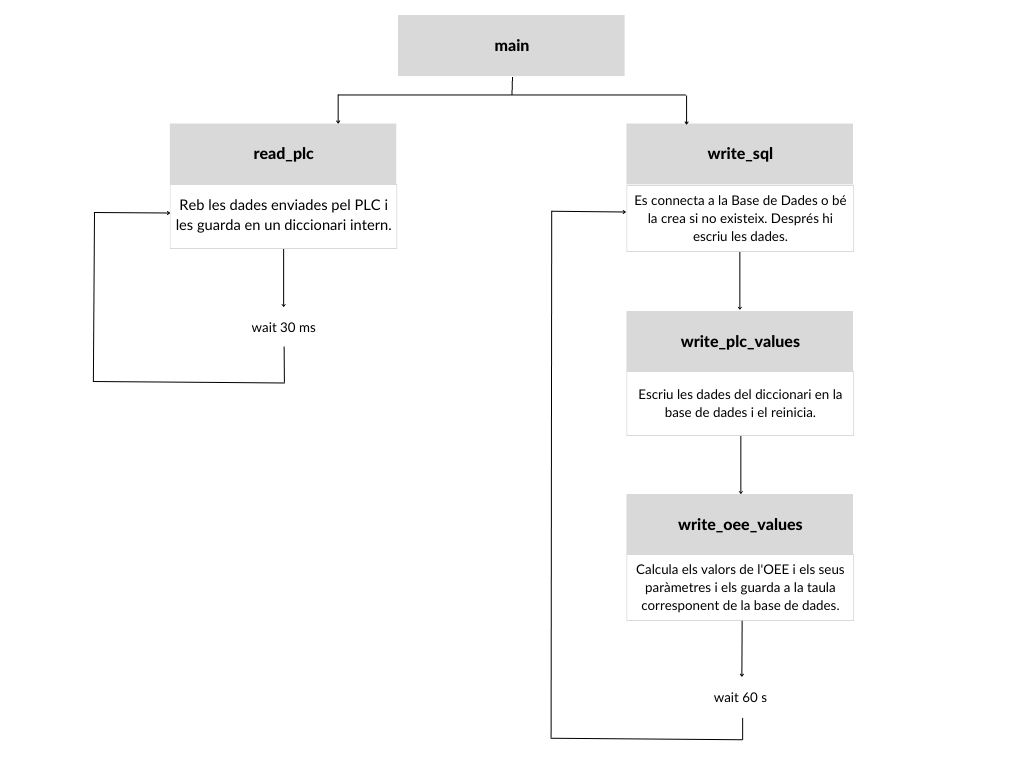
\includegraphics[width=0.5\textwidth]{img/mainProgramDiagram.png}
\caption{Esquema del funcionament del programa principal.}
\label{image:maindiagram}
\end{figure}

S'ha decidit programar les comunicacions amb el \acro{plc} i els càlculs de l'efectivitat total dels equips en un mateix mòdul. S'ha programat així perquè es fa servir la mateixa base de dades per a tots dos objectius.

D'aquesta forma, s'ha creat un programa Python amb dos fils d'execució. Un fil en Python --- també conegut com a \emph{thread} --- és una seqüència d'execució independent dins un programa que pot executar diverses tasques alhora. Així, un programa que utilitza fils té la capacitat de dur a terme diverses tasques al mateix temps, per la qual cosa permet millorar el rendiment i l'eficiència. En Python, els fils es poden crear mitjançant el mòdul \texttt{threading}. Cada fil té la seva pròpia pila d'execució, per la qual cosa són totalment independents del fil principal del programa.


S'ha de tindre en compte, però, que en alguns casos l'ús de fils mal planificat pot produir errors, com condicions de carrera o bloquejos. Una condició de carrera és un problema que ve provocat quan dos o més fils poden intentar accedir i modificar a la vegada un mateix recurs. Per exemple, un exemple de condició de carrera seria que un fil estigués llegint el valor d'una variable mentre un segon fil l'està modificant. Això provocaria que el primer fil llegís un valor incorrecte o inconsistent. Els bloquejos mutus o \emph{deadlock} es produeix en el moment que dos o més fils estan esperant que l'alliberament de recursos utilitzats per algun altre fil o programa. Això provoca que els fils es bloquegin mútuament i no puguin avançar, provocant un estancament del programa. S'ha de tindre compte amb els \emph{deadlocks} perquè sovint són difícils de detectar i solucionar, ja que solen ser aleatoris i poden provocar problemes diferents.

Tenint en compte això, s'ha creat un programa amb dos fils diferents d'execució --- Imatge \ref{image:maindiagram}. El primer fil s'encarrega de gestionar les comunicacions amb el \acro{plc} i guardar la informació rebuda en un diccionari. El segon fil gestiona la base de dades, hi escriu la informació rebuda des del \acro{plc} i els resultats que s'han calculat per obtenir l'\acro{oee}:

\begin{itemize}
    \item \texttt{read\_plc}: gestiona les comunicacions amb el \acro{plc} i guarda les dades llegides en un diccionari que serà consultat posteriorment pel segon fil. Aquest fil s'executa en un bucle sense fi cada \SI{30}{ms}.
    \item \texttt{write\_sql}: llegeix les dades del diccionari i les guarda en la taula \texttt{table\_plc} de la base de dades. Posteriorment, crida la classe \texttt{oee} per calcular l'eficiència general dels equips i guarda els resultats en la taula \texttt{table\_oee} de la base de dades. Tot això és fa en un bucle infinit una vegada per minut.
\end{itemize}

Tots els codis així com els documents d'aquest treball estan recollits en el dipòsit \texttt{\href{https://github.com/6q4598/TFG}{6q4598/TFG}} de GitHub. La seva estructura està documentada tant en un arxiu \fitx{Readme} dins del propi dipòsit com en l'apèndix \ref{anex: repo}.

\section{Programa principal}
La funció principal del programa és ben senzilla. La seva única finalitat és crear i executar els dos fils.

\begin{lstlisting}[style=Python]
def main():
    read_plc_thread = Thread(target = read_plc)
    write_sql_thread = Timer(10, function = write_sql)
    read_plc_thread.start()
    write_sql_thread.start()
\end{lstlisting}

\section{\texttt{read\_plc}}
Aquest fil llegeix les dades del \acro{plc} i les guarda en un diccionari compartit amb el fil \texttt{write\_sql}. És infinit, i es va executant recursivament cada \SI{30}{\ms}. Per tal de comprovar la robustesa del codi i veure que es llegeixen les dades correctament, s'ha programat un \acro{plc} amb un banc de proves.

\begin{figure}[h]
\centering
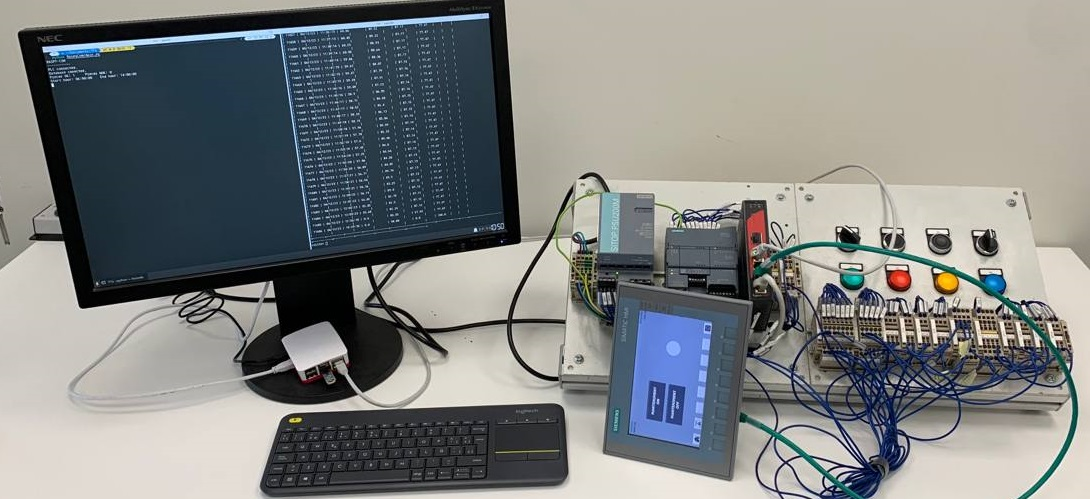
\includegraphics[width=0.5\textwidth]{img/bancProves.jpg}
\caption{El banc de probes conté un \acro{plc} Siemens SIMATIC S7-1200 amb una botonera de control i un \acro{hmi}.}
\label{s71200}
\end{figure}

\subsection{\acro{plc} i banc de proves}
Per tal de provar les comunicacions del \acro{plc} i la correcta lectura dels \emph{data block} --- d'ara endavant \acro{db} --- d'aquest, s'ha programat un banc de proves amb un \acro{plc} Siemens SIMATIC S7-1200 --- Figura \ref{s71200}. En aquest \acro{plc} s'han definit tres \acro{db}, dels quals se n'han fet servir dos. Els \acro{db} que s'han definit són el 91, el 92 i el 100. D'aquests, el 91 gestiona les dades que s'han de llegir des de la Rapsberry PI, el 92 es guarda per si en algun moment es volen enviar dades des de la Raspberry PI al \acro{plc}, i el 100 guarda una llista de tots els possibles errors que hi poden haver, que s'enviaran si hi ha hagut algun problema amb el \acro{plc} i s'ha activat el bit d'error del \acro{db} 91.

\subsubsection{\acro{db} 91}
\label{subsection:db91}
En el dB 91 s'han definit els següents bits, com es pot veure en la taula \ref{table:db91}.

\begin{table}[h]
\centering
\begin{tabular}{
>{\columncolor[HTML]{EBEAEA}}llllll}
\cellcolor[HTML]{D3D3D3} Descripció & \cellcolor[HTML]{D3D3D3} Tipus & \cellcolor[HTML]{D3D3D3} Byte &  \cellcolor[HTML]{D3D3D3} Bit \\
Automàtic & Bool & 0 & 0 \\
Manual & Bool & 0 & 1 \\
Auditoria & Bool & 0 & 2 \\
Error & Bool & 0 & 3 \\
Manteniment & Bool & 0 & 4 \\
Peça OK & Bool & 1 & 0 \\
Peça NOK & Bool & 1 & 1 \\
\end{tabular}
\label{table:db91}
\caption{Taula que mostra els bits definits en el \acro{db} 91.}
\end{table}

Els cinc primers bits corresponen al mode de funcionament del \acro{plc}, que poden ser:

\begin{itemize}
    \item Automàtic
    \item Manual
    \item Auditoria
    \item Error
    \item Manteniment
\end{itemize}

Només en el primer cas es fa el càlcul de l'\acro{oee}, mentre que els modes de \emph{manual} i \emph{auditoria} s'ignoren. El bit d'\emph{error} s'activa quan hi ha hagut algun error en la màquina, instant en el que també s'envia el codi de l'error mitjançant el \acro{db} 100. El bit de \emph{manteniment} s'ha d'activar quan hi ha algun manteniment a la màquina no planificat. Tant si el bit d'\emph{error} com si el bit de \emph{manteniment} estan actius, l'\acro{oee} ho ha de gestionar i contemplar en la disponibilitat com a $t_{e}$.

Els bits de \emph{peça ok} i \emph{peça nok} s'activen quan s'ha fabricat una peça i aquesta es dona com a bona o dolenta, respectivament. Com que el programa llegeix el \acro{db} cada \SI{30}{ms}, aquesta lectura s'ha de gestionar correctament si es volen llegir totes les peces. Per això, el \acro{plc} activa aquests bits a $1$ durant una finestra de \SI{100}{ms} per donar temps a la Raspberry PI de llegir-ho correctament --- posteriorment en la secció \ref{section: raspicom_codi} s'explicarà amb detall com es gestiona.

\subsubsection{\acro{db} 100}
Aquest \acro{db} només enviarà el codi d'error corresponent a la Raspberry PI en cas que el bit d'\emph{error} del \acro{db} 91 estigui actiu. En l'apèndix \ref{anex: db_100} hi ha la llista de tots els errors que s'han contemplat. Tanmateix, i a causa de a la limitació que ofereix el banc de proves, l'únic error que de veritat es té en compte és el primer, tots els altres s'han definit segons el que es va decidir en el seu moment aprofitant programes previs d'Ingimec, però no es fan servir. Això és així perquè tots els polsadors i selectors disponibles, així com l'\acro{hmi}, es fan servir per altres accions.

Així, els errors que s'han activat en el \acro{db} 100 s'afegeixen en una llista dins el diccionari --- secció \ref{section: raspicom_codi}. D'aquesta forma es poden afegir a la taula indicada de la base de dades.

\subsubsection{Banc de proves}
S'ha definit un banc de proves que mitjançant botons i interruptors simula ser una màquina real. El banc de proves que s'ha creat consta de les següents parts:

\begin{itemize}
    \item Dos interruptors selectors de dues posicions amb retorn, els quals gestionen el mode --- \emph{automàtic}, \emph{manual}, \emph{auditoria} o \emph{error} que es vol simular.
    \item Dos polsadors que simulen ser les peces creades. N'hi ha un per les peces <<bones>> i un altre per peces <<dolentes>>.
    \item Un panell \acro{hmi} Siemens \acro{ktp400} Basic \acro{pn}, que serveix per simular l'únic mode que no es gestiona amb els selectors: els manteniments no planificats.
\end{itemize}

Així, el primer interruptor --- començant des de l'esquerra --- activa el mode \emph{automàtic} si es gira cap a l'esquerra, o \emph{manual} en cas contrari. L'altre interruptor activa els modes d'\emph{auditoria} o d'\emph{error}.

D'altra banda, en prémer el primer polsador --- el de l'esquerra ---, s'envia una seqüència que activa el bit de \emph{peça ok} durant \SI{100}{ms} cada \SI{10}{s}. Quan es manté polsat un segon o més, la seqüència s'atura. El funcionament és el mateix per l'altre polsador, tot i que aquest activa el bit de peça dolenta. Aquest sistema fa que no hàgim de clicar el botó un nombre elevat de peces per a obtenir valors de referència adequats per al càlcul de l'\acro{oee}.

Com que en un inici no es va tindre en compte que hi poguessin haver manteniments no planificats, i ja que en el banc de proves no hi havia espai per afegir aquesta opció, es va programar un \emph{hmi} per tal de poder-ho gestionar. Aquest disposa de dos botons virtuals, els quals serveixen per activar o desactivar aquest mode, a més d'un indicador visual que serveix per saber si el mode està activat o no.

S'ha de dir, però, que quan es va programar aquest banc de proves no es van tindre en compte certes incongruències. Per exemple, es pot donar el cas que els dos selectors estiguin fora de la posició neutral, de forma que dos modes poden estar actius al mateix temps. Tampoc es va contemplar que no es poguessin enviar peces en els modes de \emph{manteniment}, \emph{auditoria} o \emph{error}. Malgrat això, i com que en la vida real això no podria passar, no es van tindre en compte aquests detalls i es va limitar a parar compte a l'hora de manipular el banc.

\begin{figure}[h]
\centering
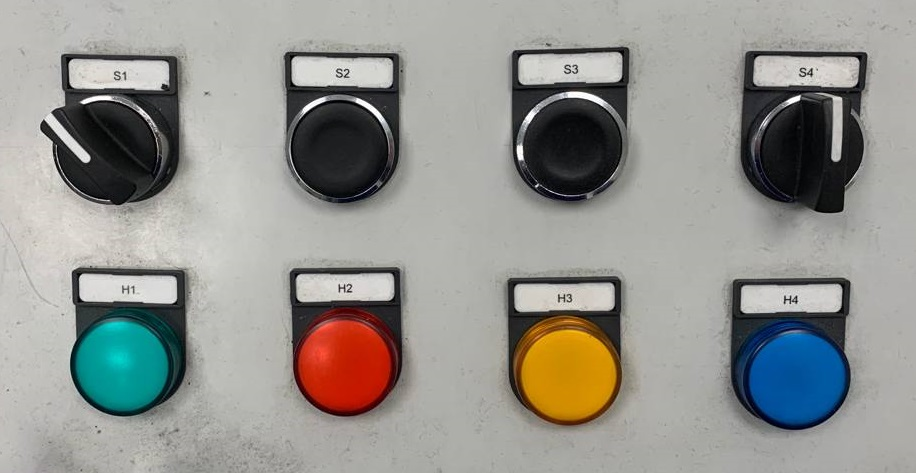
\includegraphics[height=2.5cm]{img/botonera.jpg}
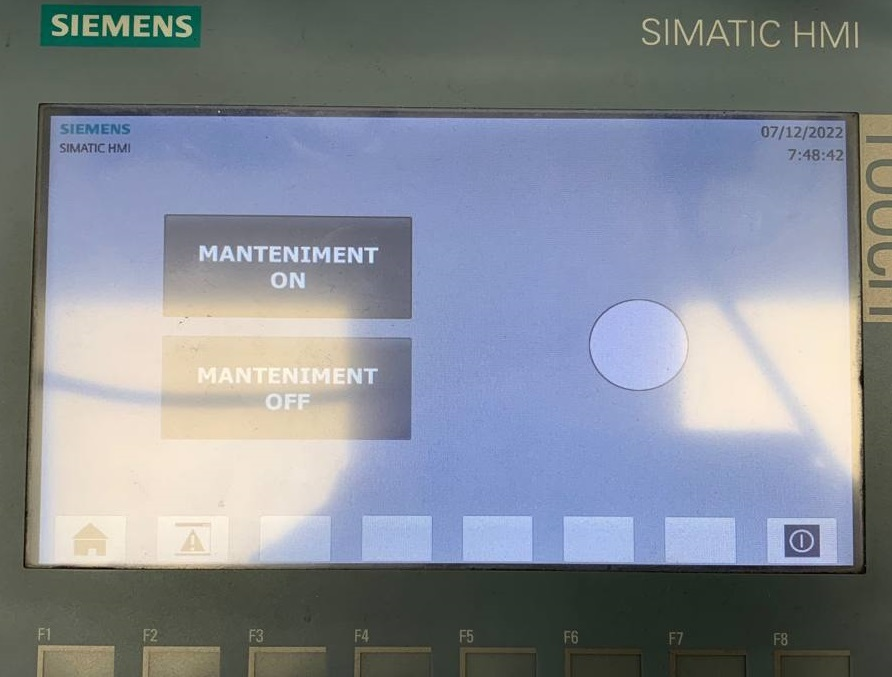
\includegraphics[height=2.5cm]{img/hmi.jpg}
\caption{Detall de la botonera i del \acro{hmi} del banc.}
\label{s71200}
\end{figure}

\subsection{Codi}
\label{section: raspicom_codi}
Per tal d'activar les comunicacions amb el \acro{plc} i poder llegir dades s'ha creat un programa Python. S'ha triat aquest llenguatge perquè és fàcil i ràpid de programar, permet crear programes amb poques línies de codi i té múltiples llibreries i paquets que faciliten la programació.

D'aquesta forma, per tal de poder comunicar la Raspberry PI amb el \acro{plc}, s'ha fet servir el paquet \texttt{python-snap7}. Aquest paquet permet les comunicacions amb els \acro{plc} de la marca Siemens.

\subsubsection{Python-snap7}
\label{section:snap7py}
Per al tema de les comunicacions, s'ha creat un programa Python que es comunica amb el PLC a través de Snap7. Snap7 és un paquet de comunicació Ethernet multiplataforma. Està disponible tant per arquitectures de 32 com de 64 bits i compta amb suport per múltiples tipus de processadors. De codi obert, permet interactuar de forma nativa amb els PLC del fabricant Siemens \cite{siemens:s7}. Tot i que ha estat dissenyat per superar les limitacions pròpies dels sistemes OPC per a transferències de gran quantitat de dades, aquesta suite s'adapta bé a petites trameses de dades com les que s'han dut a terme. Es pot trobar més documentació sobre Snap7 a \cite{snap7:documentation}.

Aquesta llibreria permet tant la lectura com l'escriptura dels PLC de la sèrie 7 de Siemens. El fet que estigui basada en \texttt{ctypes} permet accés directe a qualsevol llibreria compartida amb el sistema operatiu. Per això es pot deixar de fer \texttt{wrapper} manualment en els programes, ja que aquesta tecnologia permet escriure codi en Python pur. Es pot veure més informació i exemples de com comunicar Python amb C mitjançant aquesta tecnologia a la pàgina oficial del projecte \cite{snap7:python-snap7}. 

Per instal·lar aquest \texttt{wrapper} hem de fer-ho mitjançant \texttt{pip}.

\begin{lstlisting}[language=Bash]
pip install python-snap7
\end{lstlisting}

\subsubsection{Diccionari}
A causa del fet que el fil \fitx{read\_plc} s'executa cada \SI{30}{ms}, i a que el fil \fitx{write\_sql} ho fa a una freqüència d'una vegada per minut, s'ha hagut de trobar una forma d'emmagatzemar les dades llegides del \acro{plc}. Així, s'ha creat un diccionari que emmagatzema les dades llegides per posteriorment escriure-ho a la base de dades. Un cop guardada tota la informació, és borra tot el contingut del diccionari i es torna a començar tot el procés. La forma com és borra el diccionari i es guarden les dades s'explica amb més detall a la secció \ref{section:writesql}. El diccionari que gestiona tota la informació que es llegeix del \acro{db} $91$ és el que segueix, amb les següents parelles de clau/valor:

\begin{lstlisting}[style=Python]
db_values = {'Auto': 0,
    'Man': 0,
    'Audit': 0,
    'Error': 0,
    'Maintenance': 0,
    'Ok': 0,
    'Nok': 0,
    'ErrorCodes': []}
\end{lstlisting}

\begin{itemize}
    \item L'enter \texttt{Auto} defineix si el mode en automàtic és actiu.
    \item L'enter \texttt{Man} defineix si el mode manual és actiu.
    \item L'enter \texttt{Audit} defineix si el mode d'auditoria és actiu.
    \item L'enter \texttt{Error} defineix si hi ha algun error en el \acro{plc}.
    \item L'enter \texttt{Maitenance} defineix si s'està fent un manteniment no programat.
    \item L'enter \texttt{Ok} guarda el nombre de peces bones que s'han fabricat.
    \item L'enter \texttt{Nok} guarda el nombre de peces defectuoses que s'han fabricat.
    \item La llista \texttt{ErrorCodes} conté els errors que s'hagin pogut produir.
\end{itemize}

\subsubsection{Càlcul de les peces fabricades}
El programa llegeix les dades del PLC cada \SI{30}{ms}, com ja s'ha dit. Aquesta decisió comporta un error, i és que si s'ha fabricat una peça al cap de \SI{29}{ms} d'haver llegit les dades o si, en canvi, s'ha fabricat després de \SI{31}{ms}, aquesta no es llegirà. Per arreglar això s'ha fet una finestra, de forma que tant el bit de peça correcta com el bit de peça dolenta es mantenen en estat alt durant un temps prou llarg.

Durant les proves, s'ha comprovat que una finestra de \SI{100}{ms} és suficient per llegir la peça correctament, tot i que s'hauran de dur a terme les mesures necessàries en el codi per evitar que la mateixa peça es llegeixi diversos cops. Un comptador emmagatzemat dins del diccionari s'encarrega de guardar el nombre de peces fabricades per poder introduir-les en la base de dades quan sigui el moment.

\subsection{Fil d'execució}
El codi següent mostra tot el fil complet de lectura dels \acro{db} $91$ i $99$. Aquesta funció conté un bucle infinit que s'executa cada \SI{30}{ms}. La primera línia d'aquest crea un objecte client del paquet \texttt{snap7} que representa una connexió al \acro{plc}. Així mateix, també es fa servir per llegir-lo o interactuar-hi. Seguidament, es comprova si hi ha una connexió activa mitjançant el mètode \texttt{get\_connected()}. Aquest és un mètode de \texttt{snap7} que retorna \texttt{True} en cas que hi hagi una connexió activa, o \texttt{False} en cas contrari. En qualsevol dels dos casos imprimeix informació sobre l'estat de la connexió.

Si hi ha una connexió activa amb el \acro{plc}, activa el \emph{flag} \texttt{plc\_connected} per tal d'informar el fil \texttt{write\_sql} que pot escriure a la base de dades. Després, comença la lectura del \acro{db} 91, que es guarda en la variable \texttt{read\_plc}. El mètode propi \texttt{convert\_byte\_to\_bit()} converteix la informació llegida en un array de bits, i ho guarda en la variable \texttt{read\_plc\_bin} per tal de fer més fàcil la inclusió de tota la informació llegida en el diccionari. Aquesta es guarda segons l'especificat en la subsecció \ref{subsection:db91}.

Aquí s'ha de fer un incís en la forma de comptar les peces. Com ja s'ha dit anteriorment, quan s'activen els bits de \emph{peça ok} i \emph{peça nok} ho fan durant un instant de temps concret. Per comptar això, és crida al mètode \texttt{count\_pieces()}. Aquest mètode accepta dos paràmetres, corresponents als bits de \emph{peça ok} i \emph{peça nok}. Els paràmetres \texttt{piece\_ok} i \texttt{piece\_nok} corresponen al valor d'aquests bits. Quan hi ha un flanc de pujada --- el paràmetre és <<$1$>> ---, activa el \emph{flag} corresponent i s'incrementa una unitat el comptador de peces. Si hi ha un flanc de baixada --- el valor és <<$0$>> ---, el flag corresponent es desactiva.  El recompte de peces es du a terme mitjançant les variables \texttt{num\_ok} i \texttt{num\_nok}. L'ús de \emph{flags} permet saber si anteriorment ja hi ha hagut un flanc de pujada del bit per tal de no comptar més d'una vegada la mateixa peça. D'aquesta forma, en les dues primeres condicions s'activa el \emph{flag} si aquest està desactivat i hi ha hagut un flanc de pujada al mateix temps que es compta una peça. En les últimes dos, es desactiva el \emph{flag} corresponent si hi ha hagut un flanc de baixada i aquest està actiu. Tots els altres casos possibles s'ignoren.

Finalment, si hi ha hagut una excepció durant aquest procés, s'imprimeix un missatge d'error i es torna a executar el bucle. Així hi ha la certesa que el programa no acabi abruptament.

\begin{lstlisting}[style=Python]
def read_plc():
    """
    Read DB 91 and 100 from the PLC.
    """
    global plc_connected, num_ok, num_nok, fabricated_ok, fabricated_nok

    while True:
        client = snap7.client.Client()

        try:
            client.connect('192.168.0.1', 0, 0)

            # If client is connected to the PLC, read DB and converts it to a bit array.
            if (client.get_connected()):
            
                if plc_connected == False:
                    print("PLC connected.")
                    
                plc_connected = True
                read_plc = client.db_read(91, 0, 2)
                read_plc_bin = convert_byte_to_bit(read_plc)
                
                count_pieces(int(read_plc_bin[10]), int(read_plc_bin[9]))
                # Then, count pieces and write it to the dictionary «db_values».
                db_values.update({'Auto': int(read_plc_bin[-1]), 'Man': int(read_plc_bin[-2]), 'Audit': int(read_plc_bin[-3]), 'Error': int(read_plc_bin[-4]), 'Maintenance': int(read_plc_bin[-5]), 'Ok': num_ok, 'Nok': num_nok, 'ErrorCodes': ''})
                
            else:
                print("PLC disconnected. Trying to reconect")

        except Exception as e:
            print("Error connection PLC. Error: ", e)
            continue

        # Set a runtime delay.
        time.sleep(PLC_SLEEP)
\end{lstlisting}

\section{\texttt{write\_sql}}
\label{section:writesql}
El segon fil del programa guarda els valors llegits del \acro{plc} en la base de dades definida en el capítol \ref{chapter:database}. Després, calcula l'\acro{oee} i guarda els resultats en la taula corresponent.

La primera acció del fil és comprovar que existeixi la base de dades. Si aquesta existeix, s'estableix una connexió utilitzant la funció \texttt{connect()} del mòdul \texttt{sqlite3}. \texttt{sqlite3} és un mòdul que proporciona una API eficient per treballar amb bases de dades relacionals SQLite. En Python, aquest mòdul permet als programadors connectar-se, crear i efectuar operacions tant d'escriptura com de lectura amb aquests tipus de bases de dades. En cas que la base de dades no existeixi, la crea i crida la funció \texttt{create\_tables()}. Aquesta funció crea les taules segons el que s'ha especificat anteriorment. Tant en el primer com en aquest cas, així com si hi ha hagut alguna excepció, s'imprimeix un missatge informatiu.

Un cop s'ha connectat a la base de dades i s'han creat --- si fa falta --- les taules corresponents, es comença el bucle infinit. Aquest s'executa una vegada per minut, i només ho fa en cas que la connexió amb el \acro{plc} s'hagi establert correctament. En cas afirmatiu, es crida la funció \texttt{write\_plc\_values()}, que accepta com a paràmetres la connexió i el cursor a la base de dades. Aquest mètode copia el contingut del diccionari \texttt{db\_values} i dels comptadors de les peces \texttt{num\_ok} i \texttt{num\_nok} en llurs variables locals. Seguidament, reinicia el contingut de \texttt{db\_values} així com dels comptadors. Finalment, ho escriu a la base de dades. Aquesta funció s'ha dissenyat així per no bloquejar el diccionari o els comptadors en el procés d'escriptura a la taula, i permetre que el fil \texttt{read\_plc} no s'hagi d'esperar que aquest procés acabi.

Posteriorment, es comprova mitjançant un \emph{flag} si s'ha creat una instància de la classe \texttt{oee}. Aquesta classe calcula els valors de l'\acro{oee}, com s'explica més endavant en el capítol \ref{chapter:oee}. Si el \emph{flag} corresponent no s'ha activat, l'activa i crea una instància d'aquesta classe. Tot seguit inicialitza els següents valors mitjançant la invocació dels mètodes corresponents:

\begin{itemize}
    \item El mètode \texttt{get\_start\_shift\_time()} obté l'hora d'inici del torn segons el dia i hora actuals. Això ho fa consultant a la taula \texttt{table\_shifts} de la base de dades.
    \item D'igual forma, el mètode \texttt{get\_end\_shfit\_time()} fa el mateix per a l'hora final.
    \item Els mètodes \texttt{get\_break\_time()} i \texttt{get\_maintenance\_time()} aconsegueixen l'hora d'inici del temps de descans i dels manteniments planificats. En cas que no hi hagi un temps de descans o un manteniment planificats, aquests mètodes retornen $-1$.
    \item En últim lloc, els mètodes \texttt{get\_break\_duration()} i \texttt{get\_maintenance\_duration()} assoleixen la durada de les parades planificades o dels manteniments programats, respectivament. D'igual forma que en els dos mètodes anteriors, si no s'han planificat parades o manteniments aquestes funciones retornen $-1$.
\end{itemize}

Un cop creada la instància a aquesta classe i inicialitzats els valors, es crida el mètode \texttt{write\_oee\_values()} que accepta com a paràmetres la connexió a la base de dades, el cursor, la instància a la classe \texttt{oee} i un \emph{flag} que s'activa si hi ha hagut o no un error. D'aquesta forma, i com s'explica en el capítol \ref{chapter:oee}, en cas que hi hagi algun error en el \acro{plc} s'ignoren tant els càlculs de la productivitat com de la qualitat. Aquesta funció crida els mètodes adequats de la classe per tal de realitzar els càlculs de l'\acro{oee}. Un cop calculats, s'escriuen a la taula corresponent de la base de dades.

\begin{lstlisting}[style=Python]
def write_sql():
    """
    Write in the database the values readed from PLC and saved in the dictionary «db_values». Then, reset «db_values» values.
    """
    global num_ok, num_nok, plc_connected, trheads_list
    flag = False

    # Start DB connection. If the database not exists, create tables.
    if (os.path.exists(sql_path)):
        print("Database conected.")
        sql_connection = sqlite3.connect(sql_path)
        sql_cursor = sql_connection.cursor()
 
    else:
 
        try:
            print("Creating database.")
            sql_connection = sqlite3.connect(sql_path)
            sql_cursor = sql_connection.cursor()
            create_tables(sql_cursor)
 
        except sqlite3.OperationalError as e:
            print("Error connecting database. Error: {}\nStopping program.".format(e))

    while True:
        if (plc_connected):

            now_error = db_values['Error']

            # Insert PLC and OEE values in the database.
            write_plc_values(sql_connection, sql_cursor)

            if (flag == False):
                # Create OEE class instance.
                flag = True
                current_oee = oee(DB_SLEEP, CYCLE_TIME, sql_connection, sql_cursor)
                current_oee.get_start_shift_time()
                current_oee.get_end_shift_time()
                current_oee.get_break_time()
                current_oee.get_break_duration()
                current_oee.get_maintenance_time()
                current_oee.get_maintenance_duration()

            write_oee_values(sql_connection, sql_cursor, current_oee, now_error)

        time.sleep(DB_SLEEP)
\end{lstlisting}

Aquí s'ha de fer un incís, ja que els canvis de torn s'han de tractar com correspon. D'aquesta forma, la primera acció que es realitza en el mètode \texttt{write\_oee\_values()} és la comprovació que l'hora actual estigui dins del torn corresponent. Si, en canvi, l'hora actual està fora del torn, es tornen a iniciar els valors anteriors i es tornen a cridar els mètodes corresponents de la classe \fitx{oee} explicats en el capítol \ref{chapter:oee}, amb l'objectiu d'obtenir els nous valors per al torn següent. Per exemple, si l'hora actual és més gran que l'hora final del torn o bé --- i tot i que això sigui impossible --- l'hora actual sigui més petita que l'hora inicial d'aquest, vol dir que s'ha començat un nou torn i que, per tant, torna a cridar els mètodes anteriors per trobar els temps actualitzats. El primer bucle \texttt{if} dins del mètode \texttt{write\_oee\_values()} du a terme aquesta acció.




\chapter{Càlcul de l'OEE}
\label{chapter:oee}
La classe \texttt{oee} calcula l'efectivitat total dels equips i tots els seus paràmetres. Aquesta classe disposa de les variables i mètodes que es descriuen a continuació. Només és instanciada una vegada en el programa principal.

\section{Atributs}
La classe \texttt{oee} disposa de divuit atributs d'instància, dels quals:

\begin{itemize}
    \item Cinc corresponen a les constants que necessitem per als nostres càlculs. Venen donades generalment pel client i teòricament no es poden canviar.
    \item Sis corresponen a les dades del torn. S'obtenen directament de la base de dades i es calculen cada vegada que comença un torn nou.
    \item Quatre per cada un dels paràmetres de l'\acro{oee}. Es reinicien cada vegada que comença un torn nou.
    \item Cinc per les variables necessàries per a aquest càlcul. També s'inicialitzen en començar un nou torn.
\end{itemize}

\subsection{Constants}
En Python no existeix un tipus de variable anomenat <<constant>> com en altres llenguatges. Malgrat això, podem aconseguir el mateix efecte definint variables d'instància i nomenant-les en majúscules. D'aquesta forma s'està indicant que el seu valor no hauria de ser modificat.

La classe \fitx{oee} conté cinc constants d'instància, les quals s'inicialitzen en el mètode \fitx{__init__} de la classe. Aquest mètode accepta quatre paràmetres, corresponents als primers valors que es mostren a continuació. Les constants de la classe \fitx{oee} es poden veure a la taula \ref{table:oee_constants}.

\begin{table}[h]
\centering
\begin{tabular}{
>{\columncolor[HTML]{EBEAEA}}llllll}
\cellcolor[HTML]{D3D3D3} Nom & \cellcolor[HTML]{D3D3D3} Tipus & \cellcolor[HTML]{D3D3D3} Descripció\\
\texttt{\acro{Sql\_connection}} & \texttt{sqlite3.connect()} & És la connexió a la base de dades.\\
\texttt{\acro{Sql\_cursor}} & \texttt{sqlite3.cursor()} & Representa el cursor de la base de dades.\\
\texttt{\acro{Interval\_duration}} & \fitx{int} & Correspon a la durada entre escriptures\\
\texttt{\acro{Cycle\_time}} & \fitx{int} & És el temps de cicle de fabricació.\\
\texttt{\acro{Object\_db}} & \fitx{db()} & Objecte de la classe \fitx{db}\\ % per a poder \\
\end{tabular}
\caption{Taula que relaciona les constants de la classe \fitx{oee} amb el seu tipus.}
\label{table:oee_constants}
\end{table}

Tant \texttt{\acro{sql\_connection}} com \texttt{\acro{sql\_cursor}} es defineixen en el fil \fitx{write\_sql}, mentre que \texttt{\acro{interval\_duration}} i \texttt{\acro{cycle\_time}} són valors enters que s'ha definit també com constants en el mateix fil. \texttt{\acro{Object\_db}} és un objecte que pertany a la classe \fitx{db} i que permet realitzar consultes sense necessitat de redundar en el codi.

\subsection{Variables}
Les variables d'instància són variables que es defineixen dins d'una classe mitjançant el mètode inicialitzador. Solen estar associades amb una instància particular de la classe, per la qual cosa cada instància d'aquesta tindrà la seva pròpia còpia de la variable. Com en el codi aquesta classe només és instanciada una vegada, això no ens és rellevant.

D'aquesta forma en la classe s'han definit en total tretze variables d'instància, de les quals n'hi ha: quatre de tipus \texttt{string} corresponents a les hores d'inici i final del torn, manteniments o parades planificades --- si n'hi ha ---; dos de tipus enter que corresponen a la durada de la parada o manteniment; quatre enters per al càlcul de l'índex \acro{oee} i cada un dels seus valors i tres enters més per als càlculs interns. La taula \ref{table:oee_variables} mostra un resum d'aquestes variables i el seu tipus.

\begin{table}[h]
\centering
\begin{tabular}{
>{\columncolor[HTML]{EBEAEA}}llllll}
\cellcolor[HTML]{D3D3D3} Nom & \cellcolor[HTML]{D3D3D3} Tipus & \cellcolor[HTML]{D3D3D3} Descripció\\
\texttt{\emph{n}\_time} & \texttt{string} & N'hi ha $4$ i guarden l'hora\\
& & llegida des de la taula \fitx{table\_shifts}.\\
\texttt{\emph{n}\_duration} & \texttt{int} & N'hi ha $2$ i guarden el temps\\
& & de duració llegit de la taula \fitx{table\_shifts}.\\
\acro{Oee} paràmetres & \texttt{int} & N'hi ha $4$, una per paràmetre calculat.\\
\texttt{current\_\emph{n}} & \texttt{int} & N'hi ha tres, i corresponen\\
& & als valors necessàris per al càlcul de l'\acro{oee}.
\end{tabular}
\caption{Taula que relaciona les variables de la classe \fitx{oee} amb el seu tipus.}
\label{table:oee_variables}
\end{table}

\section{Mètodes}
Aquesta classe conté, sense comptar el mètode constructor, un total de 22 mètodes. Aquests es poden dividir, al seu torn, en tres grans categories: de modificació, de consulta i de càlcul.

Els mètodes de modificació serveixen per inicialitzar variables de la classe i es criden en començar el programa o bé un torn nou. Els mètodes de consulta fan el mateix que els anteriors, però extraient la informació de la base de dades. També solen ser més complicats, perquè han de tractar diverses condicions abans d'executar la consulta. Els mètodes de càlcul, com el seu nom indica, fan les operacions necessàries per obtenir el valor de l'\acro{oee} i els seus components.

\subsection{Mètodes de modificació}
Inicialitzen algunes de les variables i constants d'instància de la classe. Aquests són els mètodes més senzills perquè no disposen de condicions, comprovacions ni bucles. Els mètodes de consulta de la classe són:

\begin{lstlisting}[style=Python]
def set_interval_duration(self, INTERVAL_DURATION)
def set_cycle_time(self, CYCLE_TIME)
def reset_values(self)
def close_connection(self)
\end{lstlisting}

\texttt{Set\_interval\_duration(self, \acro{interval\_duration})} estableix la constant d'instància \texttt{\acro{interval\_duration}} segons el valor que se li hagi passat com a paràmetre. En els fils d'execució no es crida mai, però si en algun moment o en determinats torns ens interessa canviar-la s'ha de fer executant aquest mètode.

\texttt{set\_cycle\_time(self, \acro{cycle\_time})} fa el mateix que el mètode anterior. Com aquesta, en el programa principal no es crida mai, però està implementat per cobrir aquells casos futurs on sigui necessari.
   
\texttt{reset\_values(self)} es crida cada vegada que comença un torn nou. Mitjançant aquesta funció, les següents variables s'inicialitzen al seu valor per defecte per poder començar des de zero tots els càlculs. D'aquesta forma tenim els càlculs de l'\acro{oee} per torns.
   
\fitx{close\_connection(self)} està implementada per si en algun moment cal tancar la connexió amb la base de dades.

\subsection{Mètodes de consulta}
Aquests mètodes serveixen, com els del punt anterior, per a modificar els atributs de la classe. No obstant això, la diferència rau en el fet que aquests ho fan consultant a la base de dades. Com que hi han definits tres torns diferents --- matí, tarda o nit --- s'han de realitzar les consultes correctament. Per exemple, en els torns de matí o de tarda no hi ha problema, ja que transcorren en un mateix dia, però en els torns de nit on l'hora inicial i l'hora final estan en dies diferents fer la mateixa consulta no és possible. En concret, els mètodes de consulta de la classe són els següents:

% def get_num_iterations(self)
\begin{lstlisting}[style=Python]
def get_break_time(self)
def get_break_duration(self)
def get_maintenance_time(self)
def get_maintenance_duration(self)
def get_start_shift_time(self)
def get_end_shift_time(self)
def update_break_true(self)
def get_num_error(self)
def total_pieces_fabricated(self)
def total_pieces_ok_fabricated(self)
def total_pieces_fabricated(self)
\end{lstlisting}

En el programa principal els dos primers mètodes que es criden corresponen a \fitx{get\_start\_shift\_time(self)} i \fitx{get\_end\_shift\_time(self)}. Aquests dos mètodes obtenen l'hora d'inici i final del torn actual, respectivament. Cada vegada que s'acaba el torn i comença un torn nou es reinicien tots els atributs de la classe mitjançant el mètode \fitx{reset\_values(self)} i es tornen a aconseguir les hores d'inici i final tornant-los a cridar.

Com que típicament hi ha tres torns --- com es pot consultar a la taula \ref{table:torns} --- les consultes s'han de realitzar correctament, ja que si no s'obtenen resultats inesperats. Per posar un exemple, en els torns de matí o de tarda aquestes hores s'assoleixen extraient de la base de dades el registre que compleixi el dia, i que l'hora actual estigui compresa entre les hores inicials i finals d'aquest. En canvi, si fem el mateix per al torn de nit, hi hauria una incongruència, ja que en la taula no hi ha una \texttt{End\_time} que sigui estrictament més gran que, per exemple, les $22:00:00$.

Per corregir-ho, tots dos mètodes fan el mateix: obtenen l'hora actual i comproven que aquesta sigui superior o igual a l'hora inicial més petita de la taula i inferior a l'hora final més gran. Com que aquests són valors que no solen variar i són definits pel client, durant les proves s'ha decidit seguir la taula d'hores següent perquè moltes empreses tenen un horari de producció semblant. Si es donés el cas que un client tingués horaris de producció diferents, s'haurien de modificar aquests paràmetres.

\begin{table}[h]
\centering
\begin{tabular}{
>{\columncolor[HTML]{EBEAEA}}lll}
\cellcolor[HTML]{D3D3D3} Torn & \cellcolor[HTML]{D3D3D3} Hora d'inici & \cellcolor[HTML]{D3D3D3} Hora final\\
\\
Matí & 06:00:00 & 14:00:00\\
\\
Tarda & 14:00:00 & 22:00:00\\
\\
Nit & 22:00:00 & 06:00:00
\end{tabular}
\caption{Taula que mostra els torns i les seves hores d'inici i final.}
\label{table:torns}
\end{table}

En el codi, això es tradueix en una estructura com la de sota. Per totes dues funcions el codi segueix el mateix esquema. També realitzen les mateixes consultes però canviant el paràmetre a buscar, ja que per obtenir l'hora inicial es busca el valor màxim de la taula mentre que per a l'hora final es busca el valor més petit --- això només en els casos en què el torn sigui nocturn.

\begin{lstlisting}[style=Python]
if (current_time >= '06:00:00' and current_time < '22:00:00'):
    sql_query = "SELECT Start_time FROM table_shifts WHERE days LIKE '%{}%' AND Start_time <= '{}' AND End_time > '{}'".format(time.strftime("%A"), current_time, current_time)
else:
    sql_query = "SELECT MAX(Start_time) FROM table_shifts WHERE days LIKE '%{}%'".format(time.strftime("%A"))
\end{lstlisting}

En sortir de la condició s'executa la consulta a la base de dades mitjançant el mètode \texttt{write\_to\_db()} de la classe \fitx{db}. Posteriorment, s'inicialitzen les variables d'instància segons el resultat obtingut i tenint en compte els possibles errors. Finalment es retorna el resultat.

A continuació es criden \fitx{get_break_time(self)} i \fitx{get_maintenance_time(self)}. Aquests mètodes obtenen l'hora d'inici del descans o del manteniment programat, respectivament. Aquí la consulta és simple, ja que per convenció en un torn com a màxim només hi pot haver un descans i un manteniment. Així, sabent el dia de la setmana i l'hora d'inici del torn la consulta que s'ha de realitzar és ben simple --- la consulta que obté l'hora d'inici del manteniment programat és idèntica a aquesta només canviant el registre a obtenir: 

\begin{lstlisting}[style=sql]
sql_query = "SELECT Break_time FROM table_shifts WHERE days LIKE '%{}%' AND Start_time = '{}'".format(time.strftime("%A", self.start_shift_time)
\end{lstlisting}

Finalment, en el programa principal els dos últims mètodes que es criden abans de continuar amb l'execució són  \fitx{get_break_duration(self)} i \fitx{get_maintenance_duration(self)}. Tampoc tenen cap misteri, ja que són els mateixos mètodes que abans però obtenint valors enters.

En aquest punt cal comentar que si no s'ha definit cap temps de descans o de manteniment a la base de dades, el mètode \texttt{write\_to\_db} sempre retornarà $-1$. D'aquesta forma hi ha la certesa que no es retornen valors inesperats o errors, i que sempre podrem tractar aquests en conseqüència. Els següents mètodes a comentar es criden en el moment de fer els càlculs de l'\acro{oee}.

\subsubsection{Disponibilitat}
\label{subsection:oeeDis}
Durant el càlcul de la disponibilitat l'única consulta que es realitza és \fitx{get\_num\_error(self)}. Aquí el codi és més complex que en els mètodes anteriors, ja que s'han de distingir tres possibles casos:

\begin{itemize}
    \item Si l'hora actual és més gran o igual que les $06:00:00$ i més petita que les $22:00:00$ --- segons s'observa en la taula \ref{table:torns}.
    \item Si l'hora actual és més gran que les $22:00:00$.
    \item Si l'hora actual és menor a les $06:00:00$.
\end{itemize}

En el primer cas es fa un \fitx{count} a la taula \fitx{table\_plc} de la base de dades de tots aquells registres amb data d'avui i hora compresa entre l'hora inicial i final calculades amb els mètodes comentats a dalt. A més, s'afegeixen com a condicions: \fitx{Error = 1} i \texttt{Break = false}.

En el segon cas la consulta és més simple, ja que només comprova si l'hora actual és més gran que l'hora d'inici del torn per al dia d'avui. Les condicions anteriors d'\emph{error} i \emph{break} es mantenen.

Per últim, si cap de les condicions anteriors s'han complert significa que el torn de matí encara no ha començat. Això genera un problema, perquè significa que el torn de nit ja s'ha estès durant dos dies diferents. Llavors, la consulta que s'ha de realitzar ha de comprovar tant els registres escrits a partir de les 22:00:00 del dia anterior com els registres escrits fins l'hora actual. Això s'aconsegueix mitjançant la funció \fitx{timedelta()} de la biblioteca \fitx{datetime} de Python.

Per acabar, si cap de les condicions anteriors s'han complert, vol dir que el torn de matí encara no ha començat. Això genera un problema, perquè significa que el torn de nit ja s'ha estès durant dos dies diferents. Llavors, la consulta que s'ha de realitzar ha de comprovar tant els registres escrits a partir de les $22:00:00$ del dia anterior com els registres escrits fins a l'hora actual. Això s'aconsegueix mitjançant la funció \fitx{timedelta()} de la biblioteca \fitx{datetime} de Python.

El codi que s'aconsegueix finalment és el següent. \fitx{current\_time} és una variable local que crida la funció \fitx{strftime} del mòdul \fitx{datetime}. Per veure més informació d'aquest mòdul es pot llegir la documentació oficial \cite{pythondoc:datetime}:

\begin{lstlisting}[style=Python]
def get_num_error(self):
    current_time = datetime.now().strftime("%H:%M:%S")
    
    if ('06:00:00' <= current_time < '22:00:00'):
            sql_query = "SELECT COUNT(*) FROM table_plc WHERE Date = '{}' AND Hour >= '{}' AND Hour < '{}' AND Error = 1 AND Break = FALSE".format(time.strftime("%D"), self.start_shift_time, self.end_shift_time)

    elif (current_time >= "22:00:00"):
        sql_query = "SELECT COUNT(*) FROM table_plc WHERE (Date = '{}' AND Hour >= '{}') AND Error = 1 AND Break = FALSE".format(time.strftime("%D"), self.start_shift_time)

    else:
        sql_query = "SELECT COUNT(*) FROM table_plc WHERE ((Date = '{}' AND Hour >= '{}') OR (Date = '{}' AND Hour < '{}')) AND Error = 1 AND Break = FALSE".format((datetime.today() - timedelta(days = 1)).strftime("%D"), self.start_shift_time, time.strftime("%D"), self.end_shift_time)

    return self.object_db.write_to_db(self.sql_connection, self.sql_cursor, sql_query)
\end{lstlisting}

D'altra banda, sempre que hi ha un temps de descans o de manteniment planificat es crida la funció \fitx{update\_break\_true(self)} que actualitza l'últim registre de la taula \fitx{table\_plc} de la base de dades posant \fitx{Break = True}. La consulta que s'executa és la següent

\begin{lstlisting}[style=sql]
UPDATE table_plc SET Break = True WHERE id = (SELECT id FROM table_plc ORDER BY id DESC LIMIT 1)
\end{lstlisting}

\subsubsection{Productivitat}
\label{subsection:oeeProd}
Per al càlcul de la productivitat necessitem els valors $t_{w}$, $t_{b}$ i $t_{e}$ representats en les variables d'instància \fitx{current\_work\_time}, \fitx{current\_planned_stop\_time} i \fitx{current\_error\_time}. Aquests valors ja s'han calculat prèviament en el càlcul de la disponibilitat. També necessitem saber el total de les peces fabricades fins a l'hora actual. Aquest valor s'obté fent una consulta a la base de dades a través del mètode \fitx{total\_pieces\_fabricated(self)}.

Aquest mètode fa un sumatori dels registres \fitx{Ok} i \fitx{Nok} de la taula \fitx{table\_plc} de la base de dades. D'igual forma que en les funcions anteriors, hem de tractar com correspon els horaris definits. Per fer-ho se segueix la mateixa estructura comentada en la subsecció \ref{subsection:oeeDis}, modificant la consulta de la següent forma:

\begin{lstlisting}[style = sql]
SELECT SUM(OK + NOK) FROM table_plc WHERE condició
\end{lstlisting}

On \texttt{condició} correspon a les condicions definides dins l'estructura de control de flux que ja s'ha comentat anteriorment.

\subsubsection{Qualitat}
Per trobar la qualitat hem de saber tant el total de peces produïdes --- tan bones com dolentes --- com el total de peces bones. El total de peces fabricades comptant les bones i les dolentes s'obté a través del mètode \fitx{total\_pieces\_fabricated(self)} definit en la subsecció \ref{subsection:oeeProd}.

El total de peces bones o \emph{ok} s'obté a partir d'una funció molt similar, \fitx{total_pieces_ok_fabricated(self)}, però on canvi la consulta canvia lleugerament. Ara el sumatori no és \texttt{SUM(OK + NOK)} sinó \texttt{SUM(OK)}.

\subsection{Mètodes de càlcul}
Permeten fer els càlculs de l'\acro{oee} i els seus paràmetres. Són un total de vuit mètodes, els quals calculen l'\acro{oee}, la disponibilitat, la productivitat i la qualitat, així com totes les dades necessàries per a trobar-los. 

\begin{lstlisting}[style = Python]
def get_oee(self)
def get_availability(self)
def work_time(self)
def planned_stops_time(self)
def update_break_true(self)
def error_time(self)
def get_performance(self)
def get_quality(self)
\end{lstlisting}

\subsubsection{Disponibilitat}
La disponibilitat es calcula mitjançant tres valors que s'han d'anar actualitzant a mesura que avança el temps: el temps de treball total $t_{w}$, el temps dels descansos planificats $t_{b}$ i el temps perdut a causa dels errors i avaries $t_{e}$. Les variables d'instància \texttt{current\_work\_time}, \texttt{current\_planned\_stop\_time} i \texttt{current\_error\_time} corresponen a aquests valors.

\texttt{Current\_work\_time} és ben fàcil de calcular. Primer, la funció \fitx{work\_time(self)} troba l'hora actual. Després, resta l'hora inicial del torn de l'hora actual. L'atribut \texttt{seconds} de la classe \fitx{datetime.timedelta} inclosa dins del mòdul \fitx{datetime} retorna en segons el resultat, ja que totes les operacions que realitzen càlculs de temps utilitzen els segons com a unitat de mesura. Finalment el codi resultant és:

\begin{lstlisting}[style = Python]
def work_time(self):
    current_time = datetime.now().strftime("%H:%M:%S")
    self.current_work_time = (datetime.strptime(current_time, "%H:%M%S") - datetime.strptime(self.start_shift_time, "%H:%M%S")).seconds
    return self.current_work_time
\end{lstlisting}

La funció \fitx{planned\_stops\_time(self)} té com a objectiu calcular el temps previst de les parades i emmagatzemar-lo a la variable d'instància \fitx{current\_planned\_stop\_time}. Primerament, s'obté l'hora actual i posteriorment es realitzen els càlculs corresponents seguint els horaris definits a la taula 6.3. És important notar que es descarten les últimes hores del torn de nit, ja que segons el control de flux definit aquestes hores corresponen al temps de descans i la disponibilitat seria zero, cosa que no és correcta. En aquesta part del càlcul, s'han de distingir quatre possibles casos:

\begin{itemize}
    \item Si un manteniment planificat coincideix amb un descans.
    \item En cas que no coincideixin el manteniment previst i la parada planificada, o bé si algun d'ells no està definit.
    \item Si en el torn no hi ha ni manteniments ni parades previstes.
\end{itemize}

En el primer cas, s'incrementa \fitx{current\_planned\_stop\_time} el temps definit en la variable \texttt{interval\_duration}. Després, s'actualitza el registre \fitx{Break} de la taula \fitx{table\_plc} perquè valgui \fitx{True} i es resta una unitat tant a \fitx{maintenance_duration} com a \fitx{break\_duration}. És rellevant notar que el càlcul es deixa de realitzar en el moment que aquestes variables siguin menors que zero --- inicialment estan inicialitzades a $-1$.

En el segon cas es fa el mateix: s'incrementa \fitx{current\_planned\_stop\_time}, s'actualitza la base de dades i es descompta la variable que pertoqui. Això no obstant, es fa separadament per distingir les parades planificades dels manteniments. En l'últim cas no es realitza cap càlcul.

Tenint tot això en compte la funció queda de la següent manera:

\begin{lstlisting}[style = Python]
def planned_stops_time(self):
    current_time = datetime.now().strftime("%H:%M:%S"   
    
    # TODO - Configure according to the requirements and the shifts of the client.
    if (current_time < "22:00.00")  
    
        # We consider whether the planned stops coincide in time with the planned maitenance.
        if ((self.break_time != -1) and (current_time >= self.break_time) and (self.break_duration > -1) and (self.maintenance_time != -1) and (current_time >= self.maintenance_time) and (self.maintenance_duration > -1)):
            self.update_break_true()
            self.current_planned_stop_time += self.interval_duration;
            self.maintenance_duration -= 1
            self.break_duration -=  
            
        elif (self.break_time != -1 and current_time >= self.break_time and self.break_duration > -1):
            self.update_break_true()
            self.current_planned_stop_time += self.interval_duration;
            self.break_duration -=  
            
        elif (self.maintenance_time != -1 and current_time >= self.maintenance_time and self.maintenance_duration > -1):
            self.update_break_true()
            self.current_planned_stop_time += self.interval_duration;
            self.maintenance_duration -=    
            
    return self.current_planned_stop_time
\end{lstlisting}

El temps perdut a causa dels errors i avaries s'obté mitjançant la funció \fitx{error\_time(self)}. Aquesta funció multiplica el nombre d'errors trobat en el mètode \fitx{get\_num\_error(self)} per la variable d'instància \fitx{interval\_duration}. És important la següent condició:

\begin{lstlisting}[style = sql]
Error = 1 AND Break = FALSE 
\end{lstlisting}

Amb això s'aconsegueix ignorar els errors que puguin haver ocorregut durant una parada o un manteniment planificats. Si no es fa això, l'error se sumaria sempre i podria fer que la disponibilitat tingués valors negatius. Per exemple, si en el torn anterior s'hagués produït un error encara no solucionat --- disponibilitat seria $0$ ---, i en el torn actual ja s'estigués en temps de descans, el resultat obtingut seria negatiu, ja que es restaria al temps treballat el temps d'error, que en aquest cas seria el mateix que el temps treballat, més el temps de descans. La funció resultant és ben senzilla:

\begin{lstlisting}[style = Python]
def error_time(self):
    self.current_error_time = self.get_num_error() * self.interval_duration
    return self.current_error_time
\end{lstlisting}

La funció \fitx{get\_availability(self)} calcula la disponibilitat segons els passos descrits en el capítol \ref{Chapter: CalcReqCom}, i arrodoneix el resultat mitjançant la funció \fitx{round} a dos decimals. Si el temps de les parades planificades i dels manteniments programats és el mateix que el temps total que ha passat dençà que ha començat el torn, genera l'excepció \fitx{ZeroDivisionError} i fica la disponibilitat al $0$\%. Finalment, retorna la variable d'instància \fitx{availability}.

\subsubsection{Productivitat}
Respecte del procés de calcular la productivitat, aquest càlcul és senzill i permet fer-lo usant només dues funcions. Ja s'ha explicat en la subsecció \ref{subsection:oeeProd} com s'obtenen la suma de totes les peces fabricades fins a l'instant actual, així que només queda explicar la funció que calcula directament aquest paràmetre.

\fitx{Get\_performance(self)} obté el total de les peces fabricades, tant les bones <<\emph{ok}>> com les dolentes <<\emph{nok}>>.  Després divideix el resultat aconseguit per $t_{t}$, el qual s'obté directament. Si aquest és $0$ crida l'excepció \emph{ZeroDivisionError} i posa la productivitat al $0$\%. Si l'excepció és qualsevol altra, imprimeix un missatge d'error i fa el mateix amb la productivitat. Es pot trobar més informació sobre els errors típics de Python i com treballar amb excepcions a la documentació oficial \cite{pythondoc:errorsAndExcpetions}. A la mateixa documentació, també hi ha un apartat dedicat a explicar el funcionament d'aquesta característica i les diferents excepcions que s'hi inclouen \cite{pythondoc:listExceptions}.

Així mateix, és important notar que acabem comprovant que el resultat obtingut no sigui negatiu o superior al $100$\%. Això és degut al fet que en les proves realitzades s'ha observat que el \acro{plc} ha \emph{fabricat} algunes peces de més, de forma que hi havia registres que en lloc de tindre sis peces en total en tenien set. Com que el cicle de producció és de \SI{10}{s} per peça, això a vegades ha provocat que la productivitat fos major al $100$\%, cosa que no hauria de passar mai.

Així mateix, és important destacar que és necessari comprovar que el resultat obtingut no sigui superior al 100\% ni negatiu. Aquesta mesura es deu al fet que durant les proves realitzades s'ha observat que el controlador PLC ha produït algunes peces de més, de manera que hi havia registres que contenien set peces en lloc de les sis esperades, incloent-hi les peces correctes i les defectuoses. Això, justament pel fet que el cicle de producció és de \SI{10}{s} per peça, ha provocat que en aquests casos concrets la productivitat superi el 100\%, cosa que no tindria de passar mai.

Tenint tot això present, la funció resultant és la que segueix. És important notar que el resultat s'arrodoneix a dos decimals mitjançant la funció \fitx{round} \cite{pythondoc:round}.

\begin{lstlisting}[style = Python]
def get_performance(self):
      try:
          self.performance = round((100 * self.total_pieces_fabricated() / ((self.current_work_time - self.current_planned_stop_time - self.current_error_time) / self.cycle_time)), 2)
          
      except ZeroDivisionError:
          self.performance = 0
          
      except Exception as e:
          print('Error in "get_performance". Error: ' + e)
          self.performance = 0
          
      if (self.performance < 0): self.performance = 0
      if (self.performance > 100): self.performance = 100
      
      return self.performance
\end{lstlisting}

\subsubsection{Qualitat}
Com ja s'ha comentat, la qualitat és el resultat de dividir el total de les peces fabricades correctament pel total de peces fabricades, incloent-hi les defectuoses. Així, la funció \texttt{get\_quality(self)} retorna el resultat d'aquesta operació arrodonit a dos decimals. Igualment, gestionem les excepcions per si encara no s'han fabricat peces, ja que del contrari retornaria un resultat indefinit \cite{hopital}.

\subsubsection{Eficiència general dels equips (\acro{oee})}
Només hi ha una funció que calcula l'\acro{oee}. \texttt{Get\_oee(self)} fa el producte descrit en la secció \ref{section:oeeCalc}. Aquesta funció retorna la variable d'instància \fitx{oee} amb el resultat arrodonit a dos decimals.





\chapter{Interfície web i servidor}
\label{chapter:iuServer}
Per acomplir aquest projecte i poder visualitzar les dades de la producció i l'\acro{oee} calculats s'ha creat un servidor Flask. Aquest servidor ha de permetre visualitzar una pàgina web simple i adaptativa on es mostrin gràfiques i dades a partir de la base de dades explicada en el capítol \ref{chapter:database}. D'aquesta forma la Raspberry PI ha de contenir tant la base de dades, com el programa de comunicació amb el \acro{plc} descrit en el capítol \ref{Chapter:comPlc} com el servidor Flask amb la seva pàgina web.

Amb tot això, aquest capítol s'estructura a través de dos punts diferents:

\begin{itemize}
    \item La creació de la pàgina web i del servidor Flask.
    \item La insta\l.lació de l'entorn Linux i configuració de la Raspberry PI.
\end{itemize}

\section{Flask i aplicació web}
\label{section:webFlask}
Flask és un entorn de treball en miniatura que permet la creació d'aplicacions web de forma senzilla i eficient \cite{flask:flask}. Gràcies a la seva estructura lleugera i flexible és una eina molt popular perquè permet als desenvolupadors adaptar-lo a les seves necessitats. A diferència d'altres entorns de treball, Flask no té cap capa d'abstracció o funcionalitat incorporada, el que es tradueix en el fet que els desenvolupadors poden implementar només aquelles funcionalitats que necessiten.

Per altra banda, en el seu dia es va decidir que l'aplicació web havia de complir les següents característiques \cite{milloresProto}:

\begin{itemize}
    \item Sistema d'usuaris per controlar l'accés a l'aplicació.
    \item Calendari per marcar els dies festius de l'any.
    \item En la pàgina principal s'ha de poder escollir entre les «\emph{n}» màquines de la línia, tot i
que per culpa de què només es disposa d'un banc de proves només s'hi ha inclòs una.
    \item Així mateix, la pàgina principal ha d'incloure les gràfiques dels paràmetres calculats, de l'\acro{oee} així com les peces fabricades i la distribució del temps. També s'han de poder visualitzar cada un dels paràmetres que composen l'índex: la disponibilitat, la productivitat i la qualitat.
    \item Gràfiques que representen els mateixos paràmetres per a un torn determinat.
    \item Connectivitat amb el \acro{plc} directament a través de \acro{tcp/ip}.
    \item Connectivitat a Internet a través d'Ethernet. Per culpa de limitacions tècniques, la connectivitat a Internet s'ha dut a terme mitjançant wifi.
    \item Disseny web adaptatiu.
\end{itemize}

Tenint tot això present, s'ha volgut fer una web tan senzilla com sigui possible. S'ha triat el model \acro{spa} per al seu disseny i implementació. \acro{Spa} és l'acrònim de \emph{Single-page application}, i és una tècnica de disseny web on tota la informació és mostra en una única pàgina \cite{Flanagan:spa}. Amb aquesta metodologia s'intenta proporcionar una experiència d'usuari fluida i ràpida mitjançant la descàrrega de tot el contingut una sola vegada, enfront dels dissenys tradicionals on el contingut es va descarregant a mesura que l'usuari avança per les diferents pàgines. Així, en els dissenys \acro{spa} el contingut es carrega dinàmicament a mesura que es va requerint, ja sigui a través de les accions dels usuaris o bé mitjançant codi inserit en els mateixos recursos. Per exemple, en l'aplicació dissenyada tot el contingut \acro{html} i JavaScript es carrega una sola vegada a l'inici, però mitjançant \acro{ajax} --- acrònim per a \emph{Asynchronous JavaScript and \acro{XML}} --- es va actualitzant cada cert temps. \acro{Ajax} és una tècnica de desenvolupament web per aconseguir crear pàgines web asíncrones. D'aquesta forma el contingut web s'executa en el client al mateix temps que per sota es manté la comunicació asíncrona amb el servidor. Per trobar més informació sobre \acro{ajax} es pot consultar la web de W3Schools \cite{w3schools:ajax}.

En l'apèndix \ref{anex: iuScreenshots} es poden veure captures de pantalla de la interfície d'usuari de l'aplicació final.

\subsection{Estructura}
Com es pot observar en la imatge \ref{image:flaskStructure}, una aplicació Flask típicament s'estructura de la següent forma:

\begin{itemize}
    \item \fitx{app} o carpeta arrel, conté tots els codis \fitx{.py} i de configuració del servidor. Sol tindre un nom semblant al nom de l'aplicació creada.
    \item \fitx{templates} conté els codis \acro{html}.
    \item \fitx{static} guarda fitxers estàtics i immutables, com estils \acro{css}, JavaScript, imatges, documents, etc. Aquests se solen emmagatzemar en subcarpetes segons el seu tipus.
\end{itemize}

Així, i com que l'aplicació resultant es basa en l'estil \acro{spa} descrit abans, només s'han creat un fitxer \acro{html} i un arxiu de configuració \fitx{.py}. Per altra banda, el directori \fitx{static} conté subdirectoris per guardar la base de dades de prova, el fitxer d'estil \acro{css}, imatges i codi JavaScript.

\begin{figure}[h]
\centering
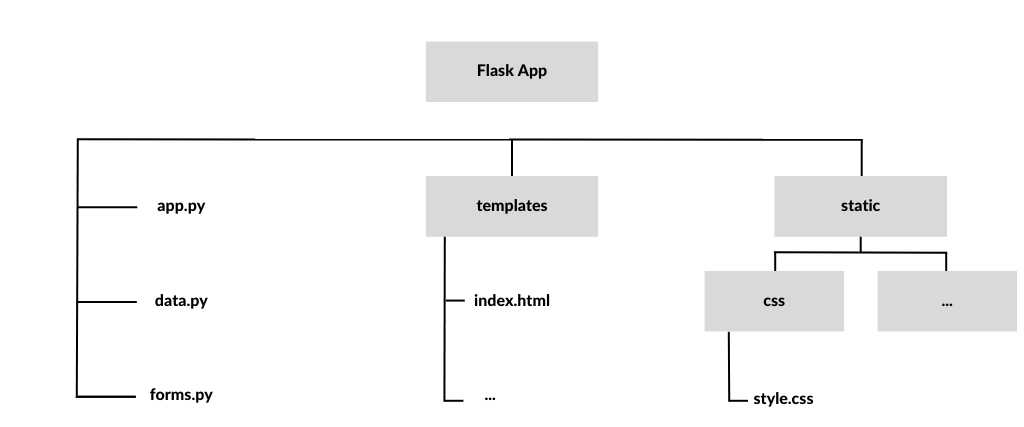
\includegraphics[width=0.8\textwidth]{img/Flask App.png}
\caption{Estructura típica d'una aplicació Flask. Diagrama basat en la secció \emph{Folder structure for a Flask app} de \texttt{\href{https://python-adv-web-apps.readthedocs.io/en/latest/flask3.html}{la web oficial del projecte}}.}
\label{image:flaskStructure}
\end{figure}

\subsection{Configuració inicial}
A causa del fet que en un inici no es disposava d'una Raspberry PI ni d'un banc de proves habilitat s'ha començat el projecte per la creació del servidor web i l'aplicació Flask. D'aquesta forma, per fer el disseny inicial i les configuracions prèvies s'ha utilitzat \emph{Windows Subsytem for Linux} o \acro{wsl} pel seu acrònim \cite{microsoft:wsl2}. Aquesta és una capa de compatibilitat pròpia dels sistemes operatius de Microsoft, la qual permet executar programes i fitxers basats en Linux sobre un sistema operatiu Windows gràcies a una interfície que simula un nucli de Linux. Tot el procés es du a terme en un entorn que no conté codi Linux i que es totalment privatiu \cite{mikegerwitz}.

S'ha iniciat la preparació de l'entorn per treballar localment en la creació del servidor. Això implica la insta\l.lació i configuració de totes les eines i \emph{plugins} necessaris. Per a tal fi, s'ha creat un fitxer \fitx{requeriments.txt} amb tots els paquets necessaris que pot ser insta\l.lat mitjançant <<pip>>. <<Pip>> és un sistema de gestió de paquets que permet la insta\l.lació, manteniment i administració d'aquests d'una forma senzilla i intuïtiva \cite{python:pip}.

\begin{lstlisting}[style = bash]
$ pip install -r requeriments.txt
\end{lstlisting}

A continuació s'explica per a què serveixen alguns d'aquests paquets. Si es vol saber més informació sobre els paquets disponibles per a aquest llenguatge, és possible consultar l'Índex de paquets de Python a \cite{python:PyPi}.

\subsubsection{Flask-Bootstrap}
\fitx{Flask-Bootstrap} és una extensió que permet integrar Bootstrap amb Flask. Bootstrap és un conjunt d'eines de codi obert que facilita el disseny de pàgines web de forma senzilla i elegant, així com una àmplia biblioteca de recursos per als desenvolupadors <<frontals>>. Aquesta extensió proporciona plantilles predefinides de Jinja2 amb elements de Bootstrap ja integrats, el que facilita la creació de llocs web moderns, sofisticats i adaptables.

\subsubsection{Flask-login}
Permet la gestió, autenticació i creació d'usuaris per aquelles aplicacions web que ho requereixin. Disposa funcions, decoradors i eines que permeten gestionar tot el procés d'autenticació d'usuaris, inicis de sessions, proteccions de rutes, validacions, etc. Amb aquest paquet també és possible personalitzar el comportament de l'autenticació per adaptar-se a la idiosincràsia de cada aplicació.

En concret, aquesta extensió permet:

\begin{itemize}
    \item Guardar l'identificador de l'usuari durant la sessió.
    \item Permetre fer inicis i finals de sessió.
    \item Permetre l'accés a certes vistes únicament als usuaris que s'hagin autentificat.
    \item Mantenir les sessions obertes inclús després que l'usuari tanqui el navegador.
    \item Protecció de les galetes de la sessió enfront tercers.
\end{itemize}

\subsubsection{Flask-SQLAlchemy, SQLAlchemy}
Aquesta extensió permet treballar amb bases de dades \acro{sql} de forma senzilla i eficient. Proporciona una capa d'abstracció sobre la base de dades, amb la que es permet de forma transparent crear models d'objectes i manipular-los mitjançant consultes. A més simplifica el desenvolupament permetent manipular objectes de la base de dades com objectes Python convencionals gràcies al fet que integra \emph{Object Relational Mapping} o \acro{orm} per les seves sigles en anglès.

\subsubsection{Flask-WTF, WTForms}
\fitx{WTForms} és una biblioteca de Python que permet crear formularis web fàcilment. Proporciona diversos tipus de validacions, així com la generació de camps de formularis personalitzats. Aquesta biblioteca pot ser integrada en aplicacions Flask mitjançant l'extensió \fitx{Flask-WTF}. Aquesta extensió proporciona protecció d'enfront atacs \acro{csrf} --- en anglès \emph{Cross-Site Reques Forgery} --- en formularis web, així com funcionalitats per a la seva validació.

\subsubsection{Jinja2}
Per la creació de llocs web dinàmics escrits en Python es pot fer servir el motor Jinja2. Jinja2 és un llenguatge basat en text, per la qual cosa es pot fer servir per generar qualsevol marcatge o codi font.

\fitx{Flask-Jinja2} és una extensió que proporciona integració amb aquest motor. Amb el seu ús, es poden configurar diverses opcions de Jinja2 en una aplicació Flask, com ara directoris de plantilles o sintaxi personalitzada, així com es permet millorar la gestió de plantilles en l'aplicació --- molt útil per futures ampliacions.

\subsubsection{WSGI}
\label{subsubsection:wsgi}
\emph{Web Server Gateway Interface} o \acro{wsgi} pel seu acrònim és una especificació que descriu la comunicació entre un servidor web i una aplicació escrita amb Python-Flask, així com la forma en què es poden arribar a encadenar diverses aplicacions. D'aquesta forma, \acro{wsgi} permet la comunicació entre el servidor i l'aplicació web actuant d'intermediari: el servidor espera peticions des de l'exterior, mentre l'aplicació fa una petició i espera que el servidor les hi passi per tal de tractar-les correctament i donar una resposta. La versió actual d'aquesta especificació és la $1.0$ segons \emph{Python Enhancement Proposals $333$} \cite{python:pepWsgi}.

Mitjançant els paquets \fitx{werkzeug} \fitx{pyuwsgi} --- es necessari tindre el servidor Apache insta\l.lat --- es proporcionen unes funcions per gestionar tasques comuns en el desenvolupament web. Algunes de les tasques que es poden gestionar amb aquest paquet són: analitzadors d'\acro{url}s, so\l.licituds d'usuaris, respostes \acro{http}, entre d'altres.

\subsubsection{Protecció CSRF}
El \acro{csrf} o \emph{Cross-site request forgery} és un \emph{exploit} maliciós d'un lloc web en el que comandes no autoritzades són transmeses per un usuari en el qual el lloc web confia. D'aquesta forma, un atac \acro{csrf} força el navegador web de la víctima a enviar una petició a una aplicació web vulnerable, la qual realitza l'acció elegida a través de la víctima. Un exemple molt clar del funcionament d'aquest <<explotador>> es recull en \cite{microsoft:csrf}.

En l'aplicació creada, la forma d'evitar aquest explotador ha estat la creació d'un testimoni únic compartit només entre el servidor i el client. D'aquesta forma, cada cop que s'envia una so\l.licitud sensible el servidor espera que contingui la clau \acro{csrf} assignada. Si aquesta clau és incorrecta, el servidor ha de rebutjar la petició. Com és obvi, per seguretat aquests testimonis no es guarden mai en les galetes del client.

\subsubsection{Werkzeug.security}
Com s'explica en \ref{subsubsection:wsgi}, \fitx{werkzeug} és un conjunt d'eines per treballar amb \acro{wsgi}. D'aquesta forma permet utilitzar-lo com la biblioteca adjacent perquè encapsula moltes funcionalitats típiques d'un entorn web. En concret, una de les funcionalitats que proporciona és el xifratge de contrasenyes mitjançant el mòdul \fitx{werkzeug.security}.

Amb això, podem fer servir les següents funcions per encriptar o desencriptar la informació dels formularis: \fitx{generate\_psw\_hash()} i \fitx{check\_psw\_hash()}.

Amb la primera generem una empremta electrònica que ha de permetre ocultar la contrasenya o altres textos que necessitem amagar. Aquesta funció accepta fins a tres paràmetres: el text de la contrasenya que es vol ocultar, el mètode d'encriptat i la longitud del \emph{salt length}, que és un valor aleatori que s'afegeix a la contrasenya per evitar que dos usuaris amb la mateixa paraula clau tinguin la mateixa empremta.

Amb la segona validem la contrasenya introduïda a través del formulari d'inici de sessió amb l'empremta electrònica guardada en la base de dades. Accepta dos paràmetres, l'<<empremta electrònica>> i el text a comparar, i retorna un valor booleà.

\subsection{Codi Python}
Aquesta aplicació la conformen tres fitxers diferents de codi Python. D'aquesta forma, \fitx{index.py} conté totes les rutes i configuracions principals de l'aplicació; \fitx{forms.py} conté les validacions dels formularis i \fitx{models.py} les crides a la base de dades i la gestió dels usuaris.

\subsubsection{\texttt{api.py}}
\label{python:codiflask}
El codi Python del fitxer \fitx{api.py} és bastant simple, ja que com s'està usant un model \acro{spa} només ha de contenir una pàgina. Així, el codi Python de la pàgina principal <<\texttt{def index()}>> només ha de cridar la funció \fitx{render\_template("index.html")} que retorna el codi \acro{html} d'aquesta, contingut en el directori \fitx{templates}.

Així mateix, i com s'explica posteriorment en la subsecció \ref{section: javascript}, per visualitzar les dades es creen rutes diferents. D'aquesta forma, per cada petició a la base de dades o gràfica a visualitzar es crea una ruta diferent. En Flask, els \emph{endpoints} són funcions que s'executen un cop el servidor rep una so\l.licitud a un \acro{url} concreta. Per crear aquestes direccions, es fa servir una sintaxi específica:

\begin{lstlisting}[style = python]
@app.route("/", methods = ["GET", "POST"]
def index():
    """
    Es realitzen les accions que requereixi la pàgina.
    """
    # Code according the app functionalities.
    # Call HTML template.
    return render_template("index.html")
\end{lstlisting}

Per cada ruta de l'aplicació es crea una funció que conté les accions que aquesta ha de realitzar. Un cop aquestes han acabat es crida el codi \acro{html} corresponent emmagatzemat dins la ruta \fitx{templates} mitjançant la funció \fitx{render\_template()}, que accepta com a paràmetre el nom del fitxer \acro{html}. Si la pàgina no ha de realitzar cap acció --- validacions de formularis, consultes a bases de dades, etc. --- es crida directament. Així mateix, aquesta funció també accepta paràmetres que posteriorment poden ser llegits i tractats en el codi \acro{html}. Mitjançant els decoradors \texttt{@app.route("nom\_de\_la\_ruta", methods = ["GET", "POST"]} s'informa el navegador que mostri la pàgina web \fitx{index.html} quan l'usuari afegeix la ruta \fitx{/} en l'\acro{uri}, així com el mètode de la petició que ha de fer. Per altra banda, es pot indicar que la mateixa pàgina sigui accessible des de dues rutes diferents afegint els decoradors necessaris a la funció.

El control d'usuaris es realitza mitjançant un formulari i Flask-Login. Aquest formulari crida la ruta \fitx{login} mitjançant el mètode \fitx{post}. Un cop s'ha validat l'accés, el formulari es deixa de mostrar i en el seu lloc es mostra un botó de \emph{logout}, el qual al seu torn crida la ruta \fitx{logout} que tanca la sessió de l'usuari. Si l'usuari ha iniciat la sessió correctament, veurà noves vistes a la pàgina principal que li permetran configurar i accedir a altres dades de la base de dades.

Per actualitzar els gràfics també s'han creat rutes diferents. D'aquesta forma, quan es vol actualitzar-ne un es crida la ruta corresponent. En el codi associat a aquesta ruta es realitzen les accions necessàries per obtenir les dades a visualitzar, les quals normalment són consultes a la base de dades.

\subsubsection{\texttt{forms.py}}
El mòdul \fitx{forms.py} conté una classe \fitx{LoginForm(Form)}. Aquesta classe hereta de la classe \fitx{Form} de Flask, per la qual cosa es fa servir per a definir un formulari d'inici de sessió. Aquesta classe defineix tres camps diferents:

\begin{itemize}
    \item \fitx{email} és un camp d'entrada de text, on els usuaris han d'ingressar el seu identificador.
    \item \fitx{psw} és un camp d'entrada de contrasenya. Això vol dir que els caràcters introduïts queden amagats a l'usuari.
    \item \fitx{remember\_login}, un camp de verificació booleà. Amb això es permet recordar l'inici de sessió.
    \item \fitx{submit}, un botó que permet enviar les dades del formulari.
\end{itemize}

Així mateix, tant \fitx{email} com \fitx{psw} tenen la validació \fitx{DataRequired()}. Amb això s'obliga a haver d'introduir tots dos camps correctament per poder realitzar l'inici de sessió. Quan es pitja el botó \fitx{submit} el formulari s'envia al servidor perquè aquest pugui processar la so\l.licitud d'inici de sessió.

\subsubsection{\texttt{models.py}}
Aquest mòdul conté les classes i funcions necessàries per gestionar els usuaris, el xifratge de les contrasenyes i les consultes a la base de dades. D'aquesta forma, \fitx{models.py} té les classes següents:

\begin{itemize}
    \item \fitx{User} conté mètodes per a xifrar la contrasenya de l'usuari.
    \item \fitx{Plc} fa les consultes a la taula \fitx{table\_plc} de la base de dades.
\end{itemize}

La classe \fitx{User} conté mètodes per xifrar la contrasenya de l'usuari. D'aquesta forma, \fitx{self\_pws(self, pasw)} crida el mètode \fitx{generate\_password\_hash(psw)} per encriptar el text passat com a paràmetre. Per la seva banda, \fitx{check\_psw(self, psw)} crida la funció \fitx{check\_psw\_hash(self, psw)} per validar la contrasenya enviada mitjançant el formulari d'inici de sessió amb l'empremta digital guardada a la base de dades.

D'altra banda, la classe \fitx{Plc} fa les crides corresponents a la base de dades per tal de poder visualitzar els gràfics correctament actualitzats. També, i si fa falta en un futur, ha de poder permetre fer canvis a la taula \fitx{table\_shfits}. De moment només s'han programat funcions amb la finalitat que facin consultes a la base de dades. Per facilitar el pas dels resultats cap al codi JavaScript que gestiona i configura les gràfiques i tota la informació que s'ha de veure, s'ha fet una crida per cada gràfica. Aquesta consulta tots els paràmetres necessaris per al gràfic en qüestió i els afegeix a una llista, que serà la que retorni finalment el mètode.

\subsection{HTML i CSS}
Per al disseny web s'han fet servir les tipografies de Google Fonts. En concret, s'ha triat la tipografia Rubik per tot el disseny, tant dels títols com dels cosos del text. D'altra banda, per al disseny frontal s'ha emprat Bootstrap. Bootstrap és una biblioteca o conjunt d'eines disponibles en diverses plataformes que permet la creació d'aplicacions web elegants i adaptables de forma senzilla. Gràcies al fet que conté plantilles, formularis, botons, requadres, menús, colors, etc. és molt senzill per als programadors crear dissenys web moderns, elegants i fàcils d'utilitzar. A diferència d'altres entorns de treball, Bootstrap només proporciona eines per al treball sobre l'aplicació frontal i no de fons com sí que fan altres biblioteques. Es pot trobar més informació sobre aquest entorn en la web oficial del projecte \cite{Bootstrap}.

En el disseny s'han fet servir diversos elements d'aquest entorn. Entre ells, un dels més importants, ja que conté el formulari d'inici de sessió i altra informació rellevant, és la barra lateral que s'estén al llarg de tota la banda esquerra de la web. En aquesta barra es mostra el logotip i informació de l'empresa, els últims valors de l'\acro{oee}, l'hora en temps real, i el formulari d'inici de sessió o botó de fi de sessió segons convingui. En concret, s'ha agafat un model d'exemple de la pàgina \cite{bootstrap:barralateral}, el qual s'ha modificat per encaixar en el disseny de l'aplicació.

Per tal de fer la pàgina web responsiva, s'han creat diverses regles \acro{css} que permeten readaptar i inclús amagar alguns elements segons la resolució de la pàgina. La forma de crear aquestes regles és mitjançant \fitx{@media}. Aquesta regla permet definir diversos estils \acro{css} per diferents mitjans o resolucions, i la seva sintaxi és:

\begin{lstlisting}[style = css]
@media screen and (max-width: 1444px) {
  #sidebar-container{
    display: none;
  }
  .graphBox {
    grid-template-columns: 1fr 1fr 1fr;
    vertical-align: middle;
    height: auto;
  }
}
\end{lstlisting}

On \fitx{screen} --- també pot ser \fitx{print} --- indica que el dispositiu en els que s'ha d'aplicar és en pantalles. \fitx{Max-width: 1444px} indica que la resolució de les pantalles on s'aplicarà aquest codi han de tindre una amplada màxima de \SI{1444}{px}. Entre les claus s'indiquen les regles que s'han d'aplicar en aquesta resolució.

Un altre punt important del codi \acro{html} és la forma d'ocultar o mostrar informació segons si un usuari ha estat validat correctament o no. Això es fa mitjançant plantilles de Jinja2. Jinja2 és un motor de plantilles per a Python configurat per defecte en Flask, de forma que facilita la separació entre l'escriptura de vistes, la lògica i la presentació. En el punt \ref{python:codiflask} ja s'ha mostrat un exemple del funcionament de Jinja2 mitjançant la funció \fitx{render\_template}. La forma de funcionar de Jinja2 és senzilla i permet el pas d'informació i de dades de forma ràpida i eficaç. Amb tot això, aquest punt s'ha realitzat mitjançant una sentència condicional com la següent:

\begin{lstlisting}[style = html]

    <!-- Contingut HTML de la Vista 1. -->

    <!-- Contingut HTML de la Vista 2. -->

\end{lstlisting}

És important notar que la sentència \fitx{if/else} està correctament escrita en Python, però que tant a l'inici com al final s'han afegit els caràcters <<\texttt{\{\%}>> i <<\fitx{\%\}}>> respectivament. Això es fa per marcar que el codi comprès entre aquests caràcters és codi Python i correspon a una sentència condicional. Per altra banda, una forma de passar paràmetres --- per exemple valors llegits de la base de dades --- és fer-ho escrivint el nom de la variable del codi Python contingut dins la funció del mòdul \fitx{api.py} entre els caràcters %\fitx{ {{ } i \fitx{ \}\} }:

\begin{lstlisting}[style = html]
<h4 style="margin-bottom: 1rem; text-align: left;">
    Welcome {{ username }}
    </h4>
\end{lstlisting}

Per altra banda, el contingut JavaScript que permet crear els gràfics interactius --- entre altres coses --- s'ha afegit a la pàgina mitjançant l'etiqueta \fitx{<script>}. A continuació es mostra un exemple real on el directori on s'ubica el codi s'indica mitjançant l'atribut \fitx{src} de l'etiqueta.

\begin{lstlisting}[style = html]
<script src = "static/sj/clock.js"></script>
\end{lstlisting}

\subsection{JavaScript}
\label{section: javascript}
Per al disseny dels gràfics i d'altres recursos, per exemple el rellotge i la data que apareixen en la barra lateral, s'ha fet servir JavaScript. Com que el contingut s'ha d'actualitzar de forma asíncrona a la resta de la pàgina, s'ha usat \acro{ajax} per a tal fi. \acro{Ajax} (\emph{Asynchronous JavaScript and \acro{xml}} és un grup de tecnologies usades per desenvolupar aplicacions web que requereixen carregar continguts de forma dinàmica i periòdica. D'aquesta forma els petits paquets de dades es bescanvien amb el servidor, per la qual cosa les pàgines web no s'han de carregar cada cop que es requereixi actualitzar la informació o que l'usuari faci una acció. Això permet que l'usuari pugui interactuar amb la pàgina sense patir les molestes interrupcions que implica haver de recarregar-la de nou, de forma que la interacció amb el servidor per part del client només es du en aquelles parts específiques que ho requereixen. Per fer un resum, \acro{ajax} es basa en les següents tecnologies \cite{ajax:ibm}:

\begin{itemize}
    \item \acro{Xhtml} i \acro{css} per presentar la informació.
    \item \acro{Dom} --- \emph{Document Object Model} ---, per visualitzar o interactuar de forma dinàmica amb el contingut.
    \item \acro{Xmlhttp}Requestper és un objecte per manipular les dades de forma asíncrona amb el servidor.
    \item \acro{Xml, html i xslt} per l'intercanvi i manipulació de dades.
    \item JavaScript per enllaçar so\l.licituds o informació.
\end{itemize}

En aquesta aplicació s'ha fet servir \acro{ajax} per actualitzar els gràfics. Aquests, al seu torn, s'han creat mitjançant Chart.js. Chart.js és una biblioteca pròpia de JavaScript que permet la creació i visualització de gràfics interactius. Mitjançant \acro{html$5$} i l'element \fitx{<canvas>} permet dibuixar gràfics adaptables fàcilment. Aquesta biblioteca permet canviar els colors dels gràfics mostrats, així com el seu tipus, ja que pot dibuixar gràfics d'àrea, de barres, de bombolles, circulars, en forma de dònut, d'àrea polar, d'aranya o de dispersió. També permet crear gràfics mixOs combinant dades i estils diferents. En la seva pàgina web \url{https://www.chartjs.org/docs/latest/} es pot trobar tota la documentació referent a aquesta llibreria.

Per al disseny de l'aplicació s'han triat dos tipus de gràfics diferents: gràfics en forma de dònut i gràfics de barres. El primer és com el circular però amb un forat al mig, i facilita la visualització de múltiples dades en un sol gràfic. El segon s'utilitza per mostrar els paràmetres de l'\acro{oee} dels torns anteriors per separat, ja que era un requisit que provenia de l'inici del projecte. Aquest es mostra horitzontalment.

Chart.js es pot insta\l.lar baixant el repositori de GitHub o fent servir els contenidors de programari \emph{cdnjs} o \emph{\acro{jsd}elivr}. Tanmateix, la forma més fàcil d'insta\l.lar-lo és utilitzar el sistema de gestió de paquets de Node.js \fitx{npm}:

\begin{lstlisting}[style = bash]
npm install chart.js 
\end{lstlisting}

Abans de poder crear gràfics s'ha d'importar la llibreria al codi \acro{html}. Per fer-ho s'usa l'etiqueta \fitx{<script>} com es descriu en la seva pàgina. És important notar que per incloure els gràfics en la interfície d'usuari s'ha de fer servir l'element \fitx{<canvas>} i assignar un identificador diferent a cada gràfic.

Per crear un gràfic amb aquesta llibreria es fa servir el següent codi, canviant els paràmetres necessaris en cada cas. Aquests són gràfics altament <<personalitzables>> on la sintaxi utilitzada per crear-los correspon al format \acro{json}. Un exemple típic és el següent.

\begin{lstlisting}[style = javascript]
 const ctx = document.getElementById('myChart');
new Chart(ctx, {
    type: 'bar',
    data: {
      labels: ['Red', 'Blue', 'Yellow', 'Green', 'Purple', 'Orange'],
      datasets: [{
        label: '# of Votes',
        data: [12, 19, 3, 5, 2, 3],
        borderWidth: 1
      }]
    },
    options: {
      scales: {
        y: {
          beginAtZero: true
        }
      }
    }
});
\end{lstlisting}

Aquest codi crea un gràfic de barres. Com que s'han fet servir gràfics en forma de dònut i de barra, podem usar tant \fitx{bar} com \fitx{doughnut} dins l'opció \fitx{type}. Dins de \fitx{labels} es pot incloure el nom de les etiquetes --- valors --- que es visualitzarà, mentre que \fitx{label} indicia el títol d'aquest i \fitx{data} conté una llista amb els valors que s'assignen. Per actualitzar els gràfics amb els valors llegits des de la base de dades s'ha fet servir una funció que crida una de les rutes definides en \fitx{api.py}. Un exemple de com es realitza aquesta acció és el següent (en l'exemple el gràfic només actualitza un valor).

\begin{lstlisting}[style = javascript]
function updateChart() {
    $.get("/route_defined_in_apipy", function(data) {
        chart.data.datasets[0].data[0] = data.datareaded;
        chart.update();
    })
}
\end{lstlisting}

En aquest exemple es defineix una funció \fitx{updateChart()} que fa servir jQuery per enviar una so\l.licitud \fitx{get} a una ruta específica definida dins del mòdul \fitx{api.py}. Un cop s'ha rebut resposta s'actualitzen les dades del gràfic existent. La funció \fitx{.get{}} de jQuery té dos arguments: el primer és la ruta a la qual s'envia la so\l.litud, mentre que el segon és una funció que s'executarà quan s'hagi rebut una resposta des del servidor. Les respostes són enviades com arguments de la funció \fitx{jsonify()} des del codi Python. Aquesta funció converteix els objectes Python en format \acro{json} mitjançant el mòdul \fitx{json}. Cada un d'aquests objectes és un element de la llista que conté els elements de la base de dades a partir de la consulta realitzada en el mòdul \fitx{models.py}. Quan hi ha una resposta des del servidor, el valor corresponent del gràfic s'actualitza. Finalment, s'envien els canvis al gràfic amb la funció \fitx{update()} de Chart.js.

Per actualitzar correctament els gràfics a intervals constants de temps es fa servir la funció \fitx{seInterval()}. Aquesta funció accepta dos paràmetres: la funció que s'ha de cridar i el temps que ha de passar entre crides --- en mi\l.lèsimes de segon.

El mateix mètode es fa servir per actualitzar els valors del rellotge digital que es veu en la barra lateral. En aquest cas no obstant es crida una funció que actualitza la data, el dia de la setmana --- gràcies a una llista---, i l'hora sense cridar una ruta predefinida. D'aquesta forma, tots els valors s'actualitzen en el mateix codi cada segon.

\section{Configuració Raspberry PI i servidor}
Per crear el servidor i fer accessible l'aplicació a través d'Internet s'ha aprofitat la Raspberry PI. La Raspberry Pi que s'ha fet servir per aquest projecte correspon a la versió $4$ Model B i té les característiques següents: 

\begin{itemize}
    \item Processador: Broadcom BCM2711 \SI{1.5}{\GHz} 64 bits Quad-Core Cortex-A72
    \item Gràfica: VideoCore VI \SI{500}{\MHz} fins a 4Kp60.
    \item Memòria: \acro{Lpddr$4$-$3200$} de 8 GB.
    \item Connectivitat: wifi a \SI{2.4}{\GHz}/\SI{5}{\GHz}, Ethernet, Bluetooth, 2 x \acro{usb} 3.0, 2 x \acro{usb} 2.0, 2 x Micro-\acro{hdmi}.
    \item Alimentació: mitjançant font externa amb connector \acro{usb-c}.
    \item Emmagatzematge: micro-\acro{sd} de 32 GB.
\end{itemize}

El sistema operatiu que s'ha insta\l.lat és un Debian 11 específic per a aquests tipus de plaques. S'ha triat aquest \acro{so} perquè és en el que està basat Raspbian, el sistema operatiu propi de l'empresa que fabrica aquestes plaques. En concret, s'ha triat l'última versió estable que hi ha disponible en \cite{debian}.

\subsection{Configuració de l'entorn}
Abans de continuar amb la configuració del servidor s'ha de preparar correctament l'entorn, ja que aquest es presenta sense interfície gràfica ni cap connexió a Internet. La configuració inicial de la placa s'ha dut a terme segons el tutorial de RaspberryTips \cite{debianInstall}. M'algrat això, per configurar tant la connexió Ethernet amb el \acro{plc} com la connexió a Internet mitjançant wifi s'han realitzat passos diferents, a causa del fet que el mètode que s'hi explica no és el més actualitzat ni el més efectiu. Per exemple, editant el fitxer \fitx{/etc/network/interfaces.d/wlan0} no és possible configurar les prioritats de xarxa, per la qual cosa la connexió a Ethernet preval sobre la connexió wifi i fa que no es pot accedir a Internet.

Per aquest motiu, les configuracions de xarxa s'han dut a terme utilitzant el programa <<\fitx{nmcli}>>. Aquesta és una eina de terminal que permet interactuar amb NetworkManager, un servei que gestiona les configuracions de xarxa de sistemes operatius basats en Linux. Amb <<\fitx{nmcli}>> es pot configurar, monitorar i visualitzar l'estat de les connexions i les xarxes del sistema. El seu ús és ben senzill, i permet configurar i visualitzar els diferents paràmetres i xarxes mitjançant l'ús de comandes. Així, el problema de seguir la pàgina anterior ha estat que la prioritat de la xarxa \fitx{eth0} corresponent al cable Ethernet era més alta que la de \fitx{wlan$0$}, corresponent al wifi --- com es pot observar en la imatge \ref{image:ipr}.

\begin{figure}[h]
\centering
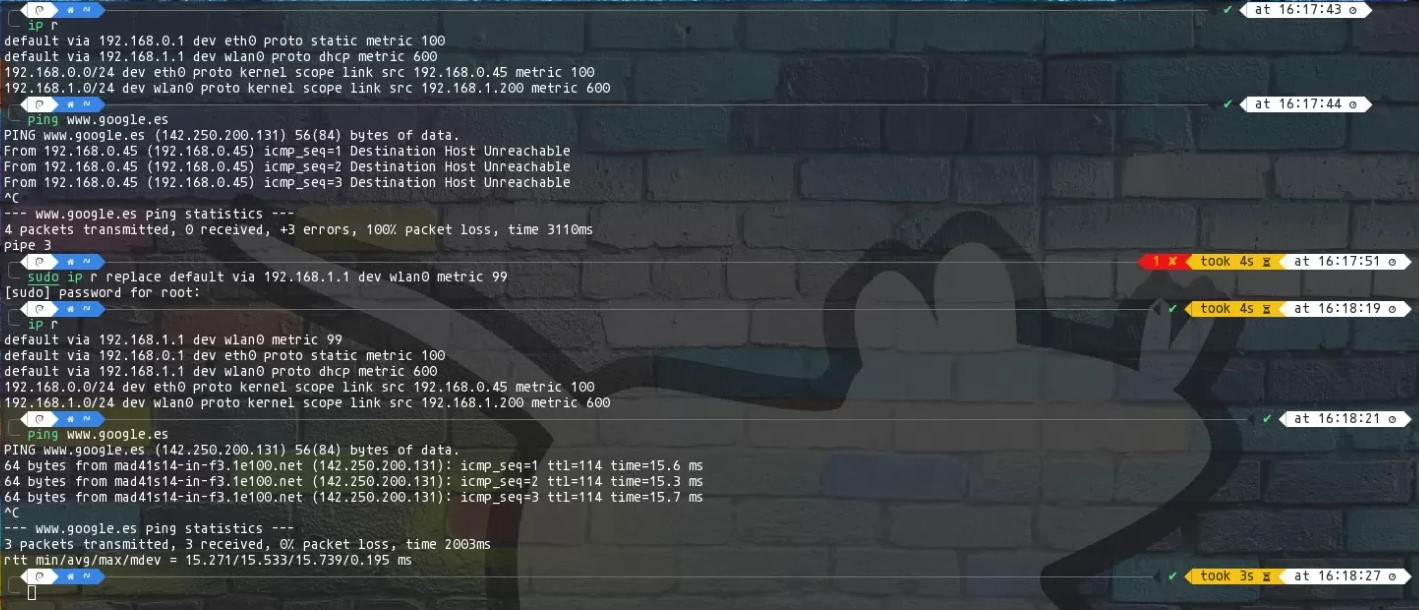
\includegraphics[width=0.8\textwidth]{img/changeInterfaceMetric.jpg}
\caption{Com es pot veure mitjançant la comanda \fitx{ip r}, la prioritat de la xarxa \fitx{eth0} és més gran que la de la xarxa \fitx{wlan0}.}
\label{image:ipr}
\end{figure}

La forma de configurar xarxes amb aquesta comanda és ben senzilla. Per exemple, per configurar Ethernet es pot fer:

\begin{lstlisting}[style = bash]
sudo nmcli c add type ethernet con-name XXX ifname eth0 ip4 YYY.YYY.YY.YY/PP gw4 yyy.yyy.yy.yy
\end{lstlisting}

On <<\acro{xxx}>> és el nom de la interfície, <<\acro{yyy.yyy.yy.yy/pp}>> és la \acro{ip} i el Port que se li vol assignar i <<yyy.yyy.yy.yy>> és la ip de la passare\l.la o porta d'entrada de la connexió. En aquest cas particular no s'ha assignat cap \acro{dns} ja que mitjançant Ethernet només s'ha de realitzar la connexió amb el \acro{plc}. Per configurar una xarxa de wifi, en canvi, ho podem fer amb aquesta altra comanda:

\begin{lstlisting}[style = bash]
sudo nmcli dev wifi con XXX password PSW
\end{lstlisting}

On <<\acro{xxx}>> és el \acro{ssid} de la wifi i \acro{psw} és la contrasenya. Per altra banda, i com s'ha explicat abans, per configurar correctament les prioritats de xarxa ho podem fer amb \fitx{ip r}.

\begin{lstlisting}[style = bash]
sudo ip r replace default via XXX.XXX.XX.XX dev wlan0 metric YYY
\end{lstlisting}

En aquesta comanda l'opció \fitx{replace} serveix per substituir una ruta existent de la taula d'encaminament; \fitx{default} indica que la ruta que s'està modificant és la per defecte; \fitx{via 192.168.0.1} indica l'adreça per on s'ha d'encaminar el tràfic de la xarxa. El paràmetre \fitx{def wlan0} fa referència al fet que el tràfic s'enviarà a través del dispositiu de xarxa \fitx{wlan0}, mentre que \fitx{metric 99} estableix la seva mètrica, que es fa servir per determinar la seva prioritat --- com menor sigui la mètrica, més gran serà. A la pàgina de \fitx{die.net} es pot trobar més informació sobre el funcionament intern de Linux \cite{linux:die}.

Una vegada s'han configurat correctament les xarxes i determinat les seves prioritats, la connexió amb la Raspberry PI s'ha realitzat tant presencialment per teclat i ratolí com mitjançant \acro{ssh}. El protocol \emph{Secure Shell} o \acro{ssh} és un protocol de xarxa que permet la connexió remota amb un altre dispositiu de forma segura perquè totes les transferències de dades estan xifrades. \acro{Ssh} permet l'ús de diversos protocols d'encriptació segons les necessitats dels usuaris. La forma d'accedir a la Raspberry PI mitjançant \acro{ssh} és executant la següent comanda en la terminal de Debian:

\begin{lstlisting}[style = bash]
ssh -p 22 pi@192.168.1.200
\end{lstlisting}

La \acro{ip} pública de la Raspberry PI és la $192.168.1.200$, l'usuari amb el qual es realitza la connexió és <<\fitx{pi}>> i aquesta es du a terme a través del port $22$, que és el port predeterminat per a les connexions \acro{ssh}.

\subsection{Configuració del servidor web}
\label{subsection: serverconfig}
Amb el Sistema Operatiu insta\l.lat, les configuracions de xarxa realitzades i establides les prioritats de les rutes és hora de triar, insta\l.lar i configurar un servidor que permeti accedir a l'aplicació Flask i a la pàgina web a través d'Internet. D'aquesta forma s'ha triat un servidor Apache per a tal fi, ja que s'ha fet servir en algunes assignatures i ja es coneix el seu funcionament \cite{apache2}.

\emph{Apache \acro{http} Server}, també conegut com a \emph{Apache Web Server} és, amb un 32.1\% de quota de mercat --- amb data d'abril de 2023 ---,  un dels servidors web més populars del món \cite{w3techs:webservers}. De codi obert i disponible per diverses plataformes, suporta una gran varietat de llenguatges de programació com \acro{php}, Python, Perl o Ruby, així com múltiples sistemes de gestió de bases de dades. Com que és un servidor software s'ha d'insta\l.lar en un servidor físic o virtual per poder oferir serveis web a través d'Internet \cite{apache}. Això vol dir que la seva principal tasca és establir la connexió i gestionar l'enviament de dades entre el servidor físic --- en aquest cas Flask --- i els clients que hi accedeixen mitjançant els seus navegadors web. Per exemple, quan un usuari accedeix a un servei web, el seu programa tramet una so\l.licitud al servidor mitjançant el protocol \acro{http} mentre Apache gestiona la consulta i la resposta des del servidor com a intermediari. Per insta\l.lar Apache a una màquina Debian es pot fer servir \fitx{apt}:

\begin{lstlisting}[style = bash]
sudo apt install apache2
\end{lstlisting}

Quan s'ha insta\l.lat, es crea el directori \fitx{/var/www} on s'ubicaran els fitxers font de l'aplicació web. Inicialment, Apache ja conté un fitxer \acro{html} de benvinguda per tal de testejar el seu funcionament. Per comprovar la insta\l.lació es pot iniciar el servidor i provar d'accedir a aquesta pàgina a través del navegador:

\begin{lstlisting}[style = bash]
service apache2 start
\end{lstlisting}

Si s'ha engegat correctament, es pot accedir a la pàgina de benvinguda a través de la \acro{ip} pública de la Raspberry PI i el port 80. Apache2 es pot configurar editant els fitxers ubicats en el directori \fitx{/etc/apache2/sites-available}. Per defecte crea dos fitxers diferents:

\begin{itemize}
    \item \fitx{000-default.conf}: estableix el contingut web que s'ha de retornar a través del port $80$, el port per defecte per a les comunicacions \acro{http}.
    \item \fitx{default-ssl.conf}: estableix la configuració per al port $443$. Aquest és el port per defecte per a les so\l.licituds \acro{https} xifrades mitjançant \acro{ssl/tls}. Com que no és segur que aquest certificat estigui insta\l.lat en un inici s'hi aplica la directiva \fitx{<IfModule mod\_ssl.c>}, que només executa la configuració si el mòdul \fitx{mod\_ssl} està carregat i disponible. Mitjançant aquest mòdul es proporciona suport per a que les connexions estiguin xifrades d'extrem a extrem.
\end{itemize}

Per a la configuració inicial de l'aplicació s'ha editat el fitxer \fitx{000-default.conf} per a comunicacions no xifrades --- més endavant, en la subsecció \ref{ssl}, es configura el protocol \acro{https} per millorar la seguretat de l'aplicació. La configuració d'Apache2 és senzilla i permet tractar el servidor i l'aplicació web separadament. D'aquesta forma la configuració del servidor s'aplica a tot el servidor web, mentre que la configuració del lloc web només s'aplica a les aplicacions web específiques. Per configurar que l'aplicació es mostri localment a través del port $80$ s'ha editat aquest fitxer de la següent forma:

\begin{lstlisting}[style = bash]
<VirtualHost *:80>
    ServerName ingiot.local
    WSGIDaemonProcess ingiot user=<pi> group=<pi> threads=5
    WSGIScriptAlias / /var/www/ingiot/ingiot.wsgi
    <Directory /var/www/ingiot/ingiot>
        Require all granted.
    </Directory>
    ErrorLog ${APACHE_LOG_DIR}/myflaskapp-error.log
    CustomLog ${APACHE_LOG_DIR}/myflaskapp-access.log combined
</VirtualHost>
\end{lstlisting}

Es pot observar que totes les peticions que entrin mitjançant el port $80$ es redirigeixen al fitxer \fitx{ingiot.wsgi}, del que se'n parla en la subsecció \ref{wsgi}. Un cop s'ha editat la configuració, s'ha d'activar mitjançant les següents comandes.

\begin{lstlisting}[style = bash]
A2enmod /etc/apache2/sites-available/000-default.conf
ls /etc/apache2/sites-enabled/
\end{lstlisting}

La primera comanda activa el fitxer de configuració, mentre que amb la segona es comprova que ho estigui llistant el contingut del directori corresponent. Si aquest hi és, es pot iniciar el servidor Apache2, o reiniciar mitjançant l'ordre \fitx{restart} si ja ho està.


\subsubsection{Especificació WSGI}
\label{wsgi}
\emph{Web Server Gateway Interface} o \acro{wsgi} és una especificació que descriu la comunicació entre un servidor i una aplicació escrita en Python. Definida dins del \acro{pep 333} \cite{python:pepWsgi}, forma part del funcionament intern d'aquest llenguatge i fa de pont entre Apache2 i Flask, convertint les so\l.licituds \acro{http} entrants al estàndard \acro{wsgi} i viceversa. Així, Flask ja conté el seu propi servidor \acro{wsgi}, encara que aquest no és capaç d'entendre múltiples peticions a la vegada, té menor rendiment i el seu ús està pensat per al desenvolupament més que per a l'aplicació final. És per això que generalment es fa ús d'altres plataformes o eines, com \emph{gunicorn}, \emph{mod\_wsgi} o \emph{u\acro{wsgi}}.

Així mateix, els servidors \acro{wsgi} disposen de servidors \acro{http} incorporats, tot i que un servidor \acro{http} dedicat sol ser més segur, eficient i capaç. El fet de posar un servidor \acro{http} enfront d'un servidor \acro{wsgi} es coneix com \emph{proxy reverse} \cite{flask:flask}. Per l'aplicació final s'ha triat fer un de \emph{mod\_wsgi} per al servei \acro{wsgi}.

El \emph{mod\_wsgi} és un servidor \acro{wsgi} integrat amb Apache. Facilita la configuració i l'inici del servidor sense necessitar escriure la configuració d'Apache. En la pàgina oficial de Flask i en la llibreria \emph{PyPI} es pot trobar més informació. Per insta\l.lar-lo és necessari un compilador i el servidor Apache, així com les capçaleres de desenvolupament. Per fer-ho, es pot utilitzar \emph{pip}:

\begin{lstlisting}[style = bash]
pip install mod_wsgi
\end{lstlisting}

La configuració d'aquesta especificació es fa mitjançant el fitxer \fitx{ingiot.wsgi} ubicat dins del directori \fitx{/var/www/}. Aquí s'ha d'indicar el directori on es troba l'aplicació web per tal de poder efectuar l'enviament de peticions correctament. D'aquesta forma, la configuració \acro{wsgi} d'aquesta aplicació queda de la forma següent:

\begin{lstlisting}[style = python]
import sys
import logging
logging.basicConfig(stream-sys.stderr)
sys.path.insert(0, "/var/ww/ingiot/ingiot/")
from app import app as application
\end{lstlisting}

D'altra banda, també s'han d'afegir tots aquells fitxers de l'aplicació necessaris perquè es puguin executar sense problemes al mateix directori.

\subsubsection{Seguretat de la capa de transport}
\label{ssl}

La <<Seguretat de la capa de transport>> o \acro{tls} --- per les seves sigles en anglès, \emph{Transport Layer Security} --- és el successor de \emph{Secure Sockets Layer} o \acro{ssl}. Aquest protocol criptogràfic permet assegurar les comunicacions realitzades a través d'una xarxa com Internet. Funciona intercanviant registres, els quals poden ser comprimits, xifrats i empaquetats amb un codi d'autenticació \acro{mac}. D'aquesta forma, cada registre conté un camp \fitx{content\_type} que especifica el protocol de nivell superior que s'està fent servir.

D'aquesta forma, un cop iniciada la connexió el nivell de registre encapsula un altre protocol: \emph{handshake} o <<Protocol d'acord>>, que al seu torn conté el \fitx{content\_type 22}. Amb això s'aconsegueix que el tant el client com el servidor enviïn diverses estructures \emph{handshake}:

\begin{enumerate}
    \item Envia un missatge \emph{ClientHello} amb una llista de tots els paràmetres de la capa, així com la versió del protocol \acro{ssl} més alta disponible. També pot enviar bytes aleatoris anomenats <<\emph{Challenge} del client>>, així com l'identificador de la sessió.
    \item El client rep un registre \emph{ServerHello}, en el qual es trien els paràmetres de la connexió a partir de les opcions oferides anteriorment.
    \item Un cop els paràmetres són coneguts client i servidor intercanvien els certificats, els quals depenen de les claus públiques de xifratge disponibles. Generalment, aquests corresponen a l'estàndard \acro{x.509}, tot i que també s'especifica l'ús de certificats \emph{OpenPGP} en un esborrany \cite{protocol:tls}.
    \item Client i servidor negocien una clau secreta simètrica anomenada \emph{master secret}. Això es pot fer mitjançant el protocol <<Diffie-Hellman>> o bé xifrant una clau secreta amb una clau pública --- que serà desxifrada amb la clau privada corresponent. Totes les dades de claus restants es calculen partint d'aquest \emph{master secret} i d'una funció pseudoaleatòria.
\end{enumerate}

Això permet dotar les aplicacions web d'una robusta capa de seguretat i xifratge que no és fàcil de vèncer. En el llibre \cite{security:compNet} es pot consultar les vulnerabilitats més comunes que poden patir els llocs web, mentre que \emph{Internet Engineering Task Force} és l'organització que elabora i publica els nous estàndards \acro{tls} \cite{protocol:tls}.

Per encriptar l'aplicació seguint aquest estàndard s'ha fet servir l'autoritat \emph{Let's encrypt}. Aquesta és una autoritat certificadora creada l'any $16$ i que proporciona certificats \acro{x.509} de forma gratuïta a través d'un mètode automatitzat dissenyat per eliminar el complex procés de creació manual que hi havia fins aquell moment. Per crear un certificat \acro{tls} mitjançant aquesta autoritat, s'ha d'insta\l.lar  el client \emph{Let's Encrypt Certbot}, que s'encarregarà de renovar automàticament el certificat i indicar el nom de domini al qual se li ha d'aplicar:

\begin{lstlisting}[style = bash]
certbot -apache -d nomdomini.com
\end{lstlisting}

S'han de seguir els passos corresponents. Per comprovar que aquest bot estigui actiu es pot fer servir \fitx{systemctl}:

\begin{lstlisting}[style = bash]
systemctl status certbot.timer
\end{lstlisting}

Amb el certificat \acro{ssl} insta\l.lat s'ha de configurar correctament Apache2 perquè accepti peticions \acro{https}. Això es pot realitzar editant el fitxer de configuració \fitx{default-ssl.conf} que es mostra en la subsecció \ref{subsection: serverconfig}.

Amb això Apache2 ja pot escoltar peticions a través del port $443$, que és el port per defecte de les peticions \acro{tls/https}. També està disponible l'opció d'afegir una redirecció amb l'objectiu que les peticions realitzades a través del port $80$ hagin de passar pel $443$.

\subsubsection{Publicació de l'aplicació web}
De moment, i com que l'aplicació no deixa de ser un prototip, no s'ha adquirit un nom de domini per a la seva publicació. Així, per a fer accessible l'aplicació a través de dispositius connectats a la mateixa xarxa s'ha enllaçat una \acro{ip} pública amb el servidor Flask. Per fer que Flask escolti a través d'aquesta \acro{ip} s'ha d'especificar dins el mètode \fitx{run}.

\subsubsection{SystemD}
Per evitar que l'aplicació falli perquè hi ha hagut un tall de corrent o s'ha reiniciat per algun motiu el dispositiu s'ha configurat \emph{SystemD}. \emph{SystemD} és un dimoni d'administració de sistema dissenyat pel nucli Linux. El nom ve del sufix \emph{System Daemon}, o processos en segon pla, i va ser desenvolupat per substituir l'anterior sistema d'arrencada d'inici \emph{init} heretat dels sistemes operatius <<System V>> i \acro{bsd} (\emph{Berkeley Software Distribution}).

Amb aquest sistema podem fer que les aplicacions s'iniciïn juntament amb el sistema operatiu, així com engegar, aturar, configurar o reiniciar serveis. Per configurar que una aplicació s'engegui amb el sistema s'ha d'editar el fitxer \fitx{/etc/systemd/system/ingiot.service}. \emph{SystemD} permet múltiples formes d'engegar les aplicacions \cite{linux:systemd}.



\chapter{Millores del prototip de cara a futures implementacions}
En la valoració final d'aquest treball, s'ha de tindre en compte que s'ha realitzat una demostració de com podria quedar la implementació final. Amb això present, es poden observar algunes mancances en el resultat final.

En primer lloc, el més fàcil seria adaptar l'aplicació web segons els criteris únics de cada client. Com es pot veure en les captures de l'annex A, no s'ha fet un treball massa acurat ni atractiu en l'aplicació web, sinó més aviat funcional. Tampoc és clar que tots els clients necessitin una aplicació responsiva, i l'estètica que s'ha definit per a l'aplicació web és millorable si es compara amb altres sistemes creats mitjançant tecnologies modernes com Grafana. Això no obstant, no s'ha volgut aprofundir més en aquest apartat, ja que només és una demostració tècnica i cada client pot tindre les seves necessitats.

Seguidament, el càlcul de l'OEE i els seus paràmetres també podria acceptar millores. Entre els conceptes definits pel client a l'inici d'aquest projecte, cap a l'any dinou, hi havia la necessitat de poder definir fins a 5 descansos diferents. En la pràctica, en canvi, s'ha decidit prescindir d'això, ja que és una petició concreta d'un client i no tots poden tindre la mateixa necessitat. En lloc d'això, s'ha decidit definir el mínim imprescindible per a un client qualsevol, i aplicar les modificacions pertinents quan sigui necessari. Així mateix, també es podria definir una hora final per als descansos i manteniments programats. Tot i que s'ha considerat que l'aplicació no s'hauria d'aturar mai, i per aquest mateix motiu no s'ha realitzat, costaria poc d'afegir i ajudaria a considerar els temps perduts a causa dels descansos i manteniments d'una millor forma, ja que passat un determinat moment aquest càlcul hauria de ser prescindible (0 en la realitat).

Una altra de les modificacions o estudis que es podrien dur a terme a futur és el fet que tot aquest treball s'ha intentat simplificar, i seria interessant estudiar com es comporten els dos fils de comunicació, així com la classe que du a terme el càlcul de l'índex \acro{oee} en altres llenguatges. És ben sabut que Python no és molt amigable amb els recursos del sistema, i les Raspberry Pi són limitades en quant aquests, així que seria interessant traslladar aquest treball en llenguatges com C o C\#, més ràpids i igual de robustos que Python.

Finalment, una de les modificacions interessants que es podria fer seria la de crear diversos bancs de treball o un de prou gran perquè simulessin una línia real de producció. Amb això es podria imitar encara més la realitat, i permetria observar millor els temps de càlcul, processat, escriptura i lectura de la Raspberry Pi. Malgrat això, i com en els casos anteriors, definir això s'ha considerat innecessari a causa del fet que Ingimec rarament dissenya dues línies similars.


\chapter{Conclusió}
\label{chapter:conclusion}
El càlcul de l'\acro{oee}, i en general la creació de sistemes que puguin calcular i mostrar en temps real la producció d'una línia, és determinant per a la indústria. No solament permet estudiar i implementar millores, sinó que facilita l'estudi de cara a futur de quins són els problemes de disseny de la línia, de forma que aquests es puguin millorar. D'aquesta forma no és d'estranyar que cada vegada més empreses dedicades al disseny, programació i muntatge de línies de producció ofereixin sistemes que permetin visualitzar de formes amigables i intuïtives aquests paràmetres.

Això no obstant, i tot i que el càlcul teòric de l'\acro{oee} és senzill, la seva implementació no ho és tant. Això és degut a causa del fet que abans de realitzar el disseny i parametritzar els càlculs s'ha de tindre clar el funcionament tant de la línia com del client, de forma que es pugui predir amb suficient encert el comportament real de la producció. En concret, aquest és un problema amb el qual personalment m'he trobat, ja que quan vaig començar a fer aquest treball tenia molts dubtes sobre quins factors eren determinants per al càlcul, i quins prescindibles. Per exemple, al començament no pensava que si la disponibilitat és penalitzada degut a algun error, no es poden penalitzar la qualitat ni la productivitat. Aquest fet un cop raonat i estudiat té tot el sentit, però en un primer moment no havia estat plantejat. D'altra banda, no només és necessari saber el temps de descans que hi ha en un torn, sinó que també ho és saber com a mínim l'hora en què aquest comença. Això s'ha sabut gràcies al fet que en les proves dutes a terme es va observar que hi havia moments en què la disponibilitat tenia percentatges negatius, cosa que no hauria de passar mai. Aquest fet es produïa, ja que la forma de calcular els temps de les parades planificades era errònia i es tenia en compte durant tot el torn (fent una regla de tres). Això provocava que si un torn començava amb un error, el temps d'aquest era igual al temps total de treball fet, fet que en ajuntar-se amb el fet de restar el temps dels manteniments o parades planificades provocava resultats negatius.

Per acabar amb la valoració dels càlculs d'aquest índex i dels seus paràmetres, també s'ha de tindre en compte que no es poden comptar les peces fabricades durant períodes de manteniment o d'error, ja que no s'hauria de tindre en compte la producció ni la qualitat en aquests moments perquè ja es penalitza la disponibilitat en el càlcul. Arribats aquí, he de donar les gràcies novament al director d'aquest treball per aconsellar-me sobre aquests punts.

Pel que respecta als temes pràctics, segurament el banc de proves no es va plantejar inicialment de la millor forma possible a causa dels errors comentats en el paràgraf anterior. Per exemple ara és sabut que no era necessari definir un bit de Manteniment o d'Auditoria, ja que en aquests casos el funcionament era el mateix que si el banc hagués estat parat perquè el càlcul d'aquest índex només es té en compte en els moments en què la producció es realitza en mode automàtic.

Així mateix, s'hagués pogut aprofitar més l'HMI per jugar i provar el prototip final amb màquines que simulessin una línia de producció real. Per exemple, es podrien afegir en aquesta pantalla botons per simular Turmats, Robots o Cintes.


En conclusió, aquest treball ha servit per aprendre sobre el funcionament de la indústria i com és de necessari per a aquest el control de la producció. També m'ha ajudat a comprendre una part important de l'enginyeria, ja que sense els enginyers de planta i els encarregats d'estudiar el seu rendiment la indústria amb tota seguretat no podria avançar a la velocitat que ho està fent.

\printbibliography

\appendix
\part{Apèndixs}


\chapter{Dipòsit del projecte}
\label{anex: repo}
Durant aquest projecte s'ha fet servir un sistema de control de versions \emph{git}. En concret, s'ha fet servir GitHub per a tal fi.  Git és un sistema de control de versions distribuït que permet el seguiment dels canvis realitzats, així com la co\l.laboració entre projectes. Per altra banda, GitHub és una plataforma web d'allotjament i gestió de projectes basada en Git. Entre altres coses, GitHub permet als usuaris crear, allotjar i col·laborar en projectes de programari lliure. D'aquesta forma, tots els codis i la documentació d'aquest treball s'han inclòs dins del dipòsit de GitHub \texttt{\href{https://github.com/6q4598/TFG}{6q4598/TFG}}.

Aquest repositori s'ha estructurat de la següent forma.

\section{\texttt{Flask}}
Conté el servidor Flask, així com la pàgina web i tots els seus fitxers. Està estructurat mitjançant els següents directoris:

\begin{itemize}
    \item \fitx{Static}: inclou tots els fitxers, imatges i recursos que es necessiten per a que la pàgina web funcioni correctament. Conté directoris on ubicar els codis \acro{css}, les imatges, els codis JavaScript i les bases de dades de test.
    \item \fitx{Templates}: inclou els codis \acro{html} de la web.
\end{itemize}

El codi del servidor està directament ubicat a dins d'aquest directori i no en una subcarpeta.

\section{\texttt{PreviousWork}}
Guarda tota la investigació prèvia sobre \acro{.net}, \acro{mvc}, Dockers, Cosmos DB etc. Al final es va decidir fer-ho tot amb Flask i Python, amb una Raspberry PI, pel que això es va rebutjar.

Aquest directori està estructurat de la següent manera:

\begin{itemize}
    \item \fitx{ApiNet}: conté tots els projectes que es van crear de nou quan encara s'intentava fer tot mitjançant \acro{.net} i \acro{mvc}.
        \begin{itemize}
            \item \fitx{IOT4246}
            \item \fitx{IOT4246\_mvc}
            \item \fitx{Screenshots}
        \end{itemize}
    \item \fitx{ArduinoCode}: amb els codis de la \acro{esp32} que es van fer en el seu moment. Aquests es van programar mitjançant Arduino IDE.
        \begin{itemize}
            \item libraries
            \item sketchEsp32Linux
        \end{itemize}
    \item \fitx{BackupsDatabase}: on s'ubiquen les còpies de seguretat de les bases de dades.
    \item \fitx{Documents}: Documents i treballs obert que m'han servit de referència.
    \item \fitx{Esp32LinuxSockets}: En cert moment, es va voler fer un programa que des de la Raspberry PI rebés les dades enviades des de l'\acro{esp32} i ho guardés en una base de dades relacional.
\end{itemize}

Dins aquest directori també s'inclouen alguns apunts interessants sobre Dockers i altres tecnologies, així com esborranys d'aquesta memòria.

\section{\texttt{RaspyCom}}
Amb els fils de comunicació amb el PLC, i d'escriptura a la base de dades. També conté la classe que fa el càlcul de l'OEE i tots els seus paràmetres.

\begin{itemize}
    \item \fitx{util}: és l'única carpeta que conté aquest directori, i és el calaix de sastre on s'han guardat totes les proves que s'han realitzat.
    \item \fitx{main.py}
    \item \fitx{oee.py}
    \item \fitx{db.py}
\end{itemize}



\chapter{Mapejat memòria del DB 100}
\label{anex: db_100}
En el \acro{db} 100 s'han definit els següents bits --- taula \ref{table:db100} --- segons el que es va decidir en l'origen del projecte:

\begin{table}[h]
\centering
\begin{tabular}{
>{\columncolor[HTML]{EBEAEA}}llllll}
\cellcolor[HTML]{D3D3D3} Descripció & \cellcolor[HTML]{D3D3D3} Tipus & \cellcolor[HTML]{D3D3D3} Byte &  \cellcolor[HTML]{D3D3D3} Bit \\
Error fusibles 24v exterior & Bool & 0 & 0 \\
Error fusibles 24v seguretat& Bool & 0 & 1 \\
Fallo Modulo emergencias & Bool & 0 & 2 \\
Fallo Modulo Barreras& Bool & 0 & 3 \\
Fallo Puertas& Bool & 0 & 4 \\
Fallo Termico Bomba Encebado& Bool & 0 & 5 \\
Fallo Presostato & Bool & 0 & 6 \\
Dispositivo profinet IFM en error 204KF1& Bool & 0 & 7 \\
Dispositivo profinet SMC en error 206K1& Bool & 1 & 0 \\
Conexión PC perdida& Bool & 1 & 1 \\
Test anulado por el usuario& bool & 6 & 2 \\
Modelo no corresponde parametros introducidos& bool & 6 & 3 \\
Medidas bomba incorrecta& bool & 6 & 4 \\
Error lectura lector intensidad 230& Bool & 9 & 7 \\
Error lectura lector intensidad 400& Bool & 10 & 0 \\
Error lectura variador 230v& Bool & 10 & 1 \\
Error lectura variador 400v& Bool & 10 & 2 \\
Error escritura lector intensidad 230& Bool & 10 & 3 \\
Error escritura lector intensidad 400& Bool & 10 & 4 \\
Error escritura variador 230v& Bool & 10 & 5 \\
Error escritura variador 400v& Bool & 10 & 6 \\
Variador en error 230& Bool & 10 & 7 \\
Variador en error 400& Bool & 11 & 0 \\
Cilindro Cierre Vertical A1.1 - \\Tiempo máximo movimiento a origen& Bool & 12 & 3 \\
Cilindro Cierre Vertical A1.1 -\\Tiempo máximo movimiento a trabajo& Bool & 12 & 4 \\
Cilindro CierreVertical A1.1 -\\Sensores detectan a la vez& Bool & 12 & 5 \\
Cilindro CierreVertical A1.1 -\\Posición perdida& Bool & 12 & 6 \\
Cilindro CierreHorizontal A1.2 -\\Tiempo máximo movimiento a origen& Bool & 12 & 7 \\
Cilindro CierreHorizontal A1.2 -\\Tiempo máximo movimiento a trabajo& Bool & 13 & 0 \\
\end{tabular}
\end{table}
\begin{table}[h]
\centering
\begin{tabular}{
>{\columncolor[HTML]{EBEAEA}}llllll}
\cellcolor[HTML]{D3D3D3} Descripció & \cellcolor[HTML]{D3D3D3} Tipus & \cellcolor[HTML]{D3D3D3} Byte &  \cellcolor[HTML]{D3D3D3} Bit \\
Cilindro CierreHorizontal A1.2 -\\Sensores detectan a la vez& Bool & 19 & 7 \\
Cilindro CierreHorizontal A1.2 -\\Posición perdida& Bool & 20 & 0 \\
Cilindro CierreHorizontalPurgador A1.3 -\\Tiempo máximo movimiento a origen& Bool & 27 & 0 \\
Cilindro CierreHorizontalPurgador A1.3 -\\Tiempo máximo movimiento a trabajo& Bool & 27 & 1 \\
Cilindro CierreHorizontalPurgador A1.3 -\\Sensores detectan a la vez& Bool & 27 & 2 \\
Cilindro CierreHorizontalPurgador A1.3 -\\Posición perdida& Bool & 27 & 3 \\
Cilindro DesplazamientoCarro A1.4 -\\ Tiempo máximo movimiento a origen& Bool & 27 & 4 \\
Cilindro DesplazamientoCarro A1.4 -\\Tiempo máximo movimiento a trabajo& Bool & 27 & 5 \\
Cilindro DesplazamientoCarro A1.4 -\\Sensores detectan a la vez& Bool & 27 & 6 \\
Cilindro DesplazamientoCarro A1.4 -\\Posición perdida& Bool & 27 & 7 \\
Cilindro BloqueoCarro A1.5 -\\ Tiempo máximo movimiento a origen& Bool & 28 & 0 \\
Cilindro BloqueoCarro A1.5 -\\Tiempo máximo movimiento a trabajo& Bool & 28 & 1 \\
Cilindro BloqueoCarro A1.5 -\\Sensores detectan a la vez& Bool & 28 & 2 \\
Cilindro BloqueoCarro A1.5 -\\Posición perdida& Bool & 28 & 3 \\
Cilindro Puerta A1.6 -\\ Tiempo máximo movimiento a origen& Bool & 28 & 4 \\
Cilindro Puerta A1.6 -\\Tiempo máximo movimiento a trabajo& Bool & 28 & 5 \\
Cilindro Puerta A1.6 -\\Sensores detectan a la vez& Bool & 28 & 6 \\
Cilindro Puerta A1.6 -\\Posición perdida& Bool & 28 & 7 \\
Valvula Entrada AH01 A2.1 -\\Tiempo máximo movimiento a origen& Bool & 29 & 0 \\
Valvula Entrada AH01 A2.1 -\\Tiempo máximo movimiento a trabajo& Bool & 29 & 1 \\
Valvula Entrada AH01 A2.1 -\\Sensores detectan a la vez& Bool & 29 & 2 \\
Valvula Entrada AH01 A2.1 -\\Posición perdida& Bool & 29 & 3 \\
Valvula Entrada AH02 A2.2 -\\Tiempo máximo movimiento a origen& Bool & 29 & 4 \\
\end{tabular}
\end{table}
\begin{table}[t]
\centering
\label{table:db100}
\begin{tabular}{
>{\columncolor[HTML]{EBEAEA}}llllll}
\cellcolor[HTML]{D3D3D3} Descripció & \cellcolor[HTML]{D3D3D3} Tipus & \cellcolor[HTML]{D3D3D3} Byte &  \cellcolor[HTML]{D3D3D3} Bit \\
Valvula Entrada AH02 A2.2 -\\Tiempo máximo movimiento a trabajo& Bool & 29 & 5 \\
Valvula Entrada AH02 A2.2 -\\Sensores detectan a la vez& Bool & 29 & 6 \\
Valvula Entrada AH02 A2.2 -\\Posición perdida& Bool & 29 & 7 \\
Ejecución alcanzado& Bool & 30 & 0 \\
Falla definida por el usuario 1& Bool & 30 & 1 \\
Fallo definido por el usuario 2& Bool & 30 & 2 \\
Tiempo de encendido alcanzado& Bool & 30 & 3 \\
Pérdida de carga& Bool & 30 & 4 \\
Feedback PID perdido durante la carrera& Bool & 30 & 5 \\
Tiempo de espera límite de corriente rápida& Bool & 30 & 6 \\
Fallo esclavo en la sincronización de velocidad& Bool & 30 & 7 \\
\end{tabular}
\caption{Taula que mostra els bits definits en el \acro{db} 100.}
\end{table}

\chapter{Captures de pantalla de l'aplicació web}
\label{anex: iuScreenshots}

\begin{figure}[h]
\centering
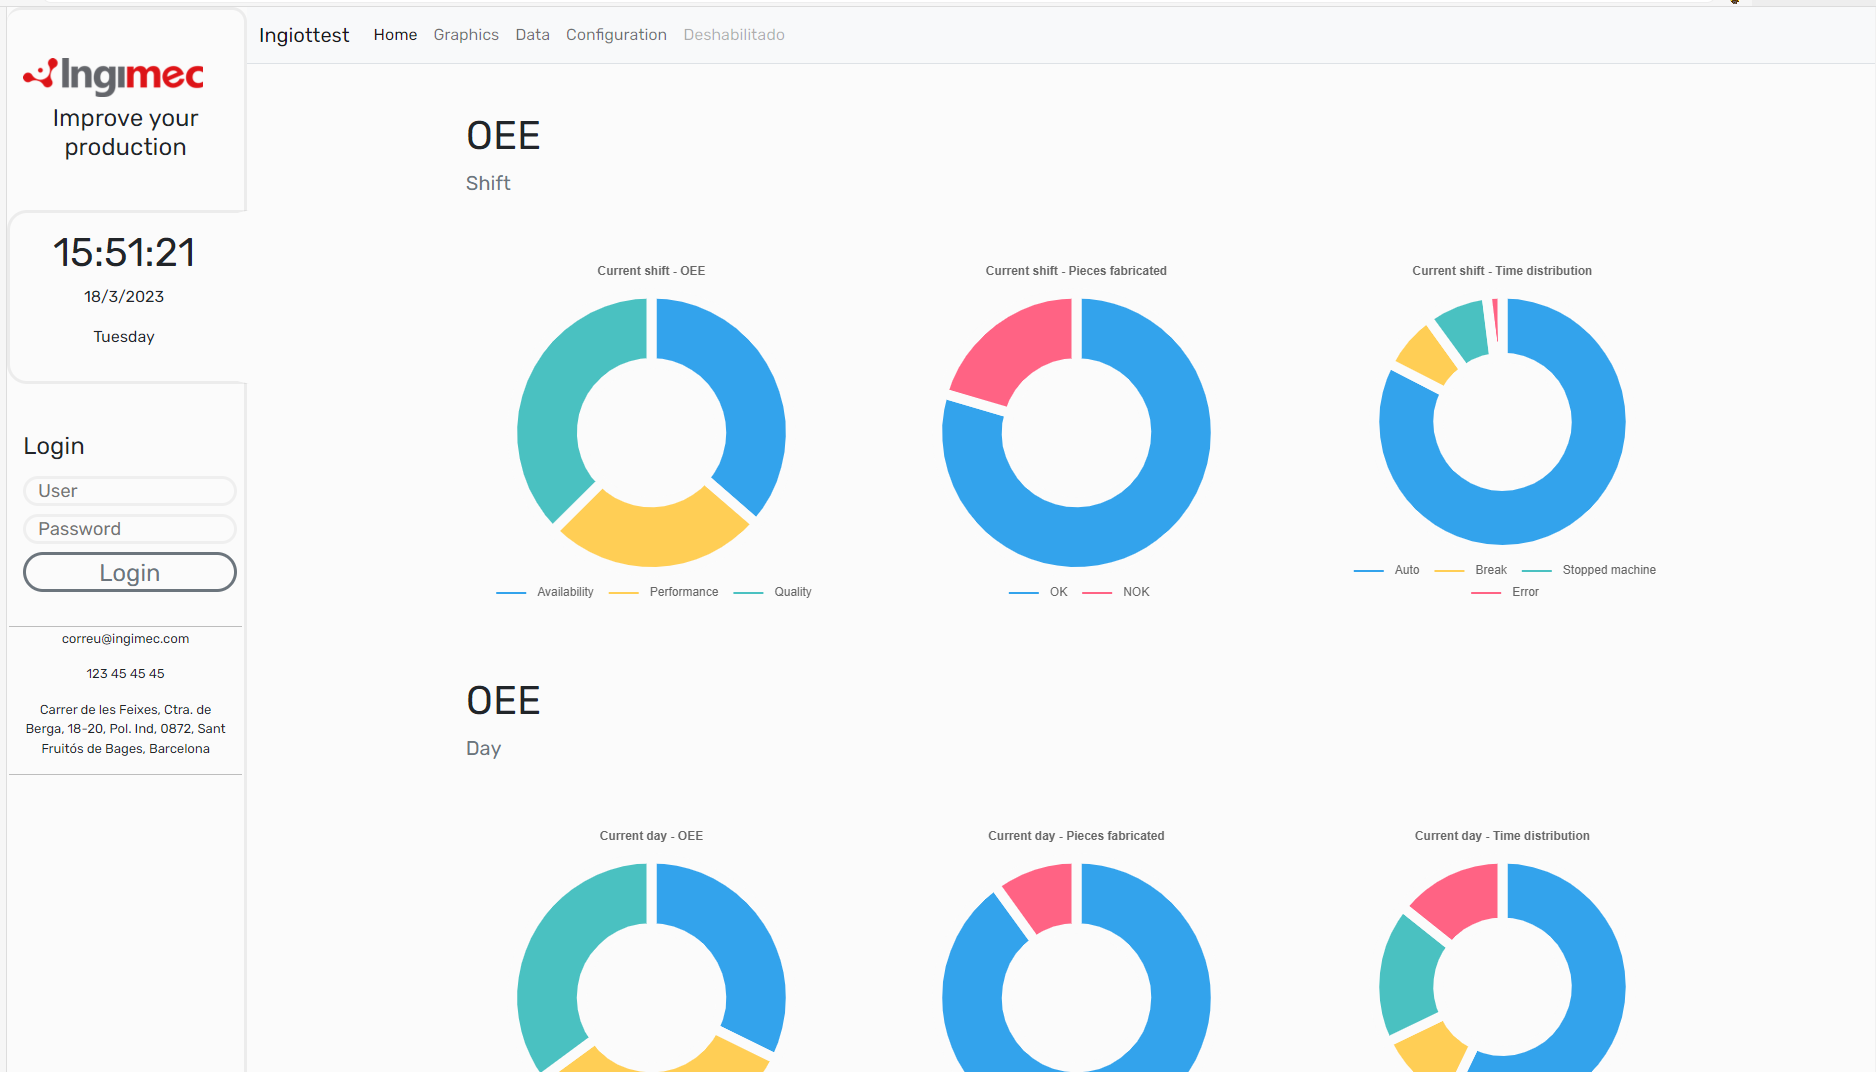
\includegraphics[width=10cm]{img/webScreenshot01.png}
\caption{Captura 1. Es mostren els valors calculats tant per al torn com per al dia actuals.}
\label{webScreen01}
\end{figure}


\begin{figure}[h]
\centering
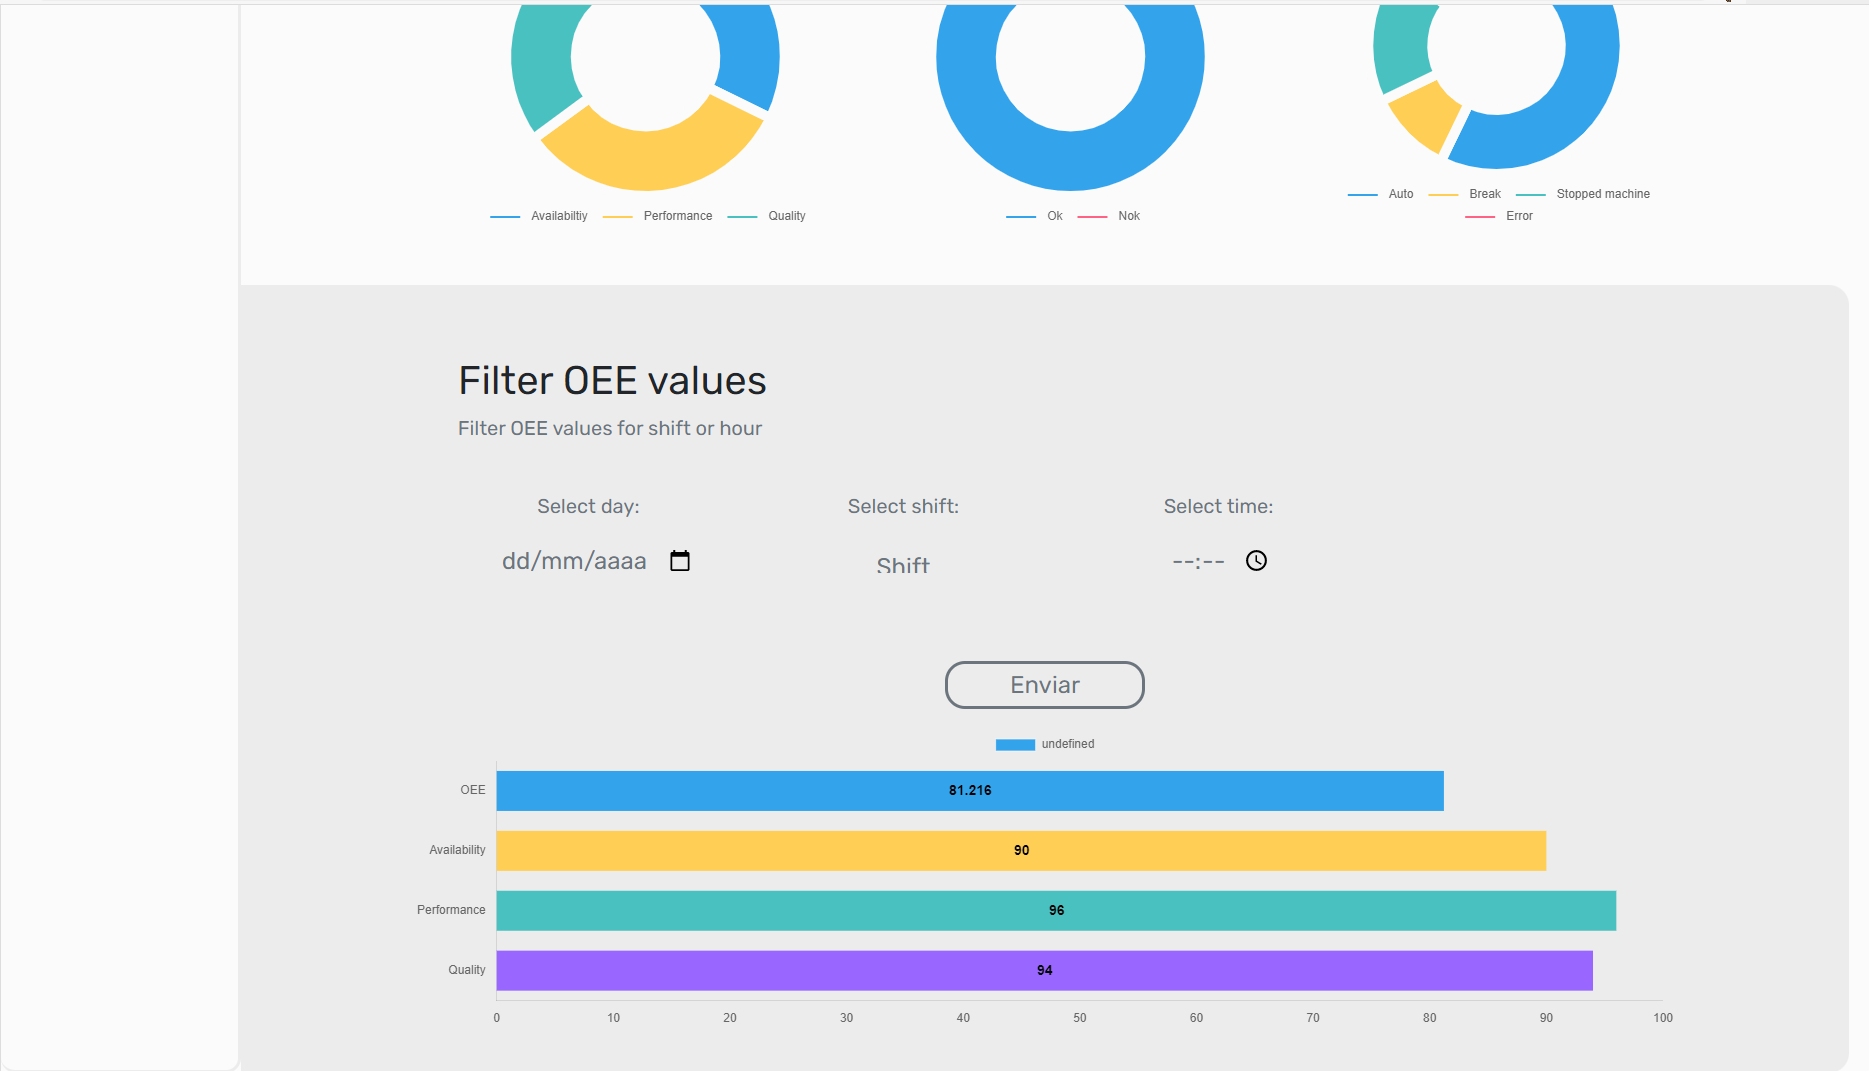
\includegraphics[width=10cm]{img/webScreenshot02.png}
\caption{Captura 2. Es permet consultar els valors de l'\acro{oee} per a un torn qualsevol de la base de dades.}
\label{webScreen02}
\end{figure}

\end{document}